%!TEX program = xelatex
\documentclass[12pt, a4paper, openany, twoside]{book}
\usepackage{pdflscape} %它在 lscape宏包的基础上增加了对通过 PDFLaTeX 方式生成 PDF 文件的支持。
     
% 字体配置文件
% % 英文字体设置特别推荐方案(Windows,需要安装 Adobe 字体),现代
% \usepackage{fontspec}
% \usepackage{xltxtra,xunicode}
% \usepackage[CJKnumber,CJKchecksingle,BoldFont]{xeCJK}
% \usepackage{xeCJKfntef}
% \usepackage{amsmath}
% \usepackage{amssymb}
% \setmainfont[Mapping=tex-text]{Times New Roman}
% \setsansfont[Mapping=tex-text]{Arial} 
% \setmonofont{Consolas}


% 英文字体设置方案一(Windows,需要安装 LM10 字体),和 LaTeX 默认字体保持一致,经典
% \usepackage{amssymb}
% \usepackage{fontspec}
% \usepackage{amsmath}
% \usepackage[CJKnumber,CJKaddspaces,CJKchecksingle,BoldFont]{xeCJK}
% \usepackage{mathrsfs}   % 一种常用于定义泛函算子的花体字母,只有大写。
% \usepackage{bm}         % 处理数学公式中的黑斜体的宏包
% \setmainfont{LMRoman10-Regular}
% \setsansfont{LMSans10-Regular}
% \setmonofont{LMMono10-Regular}

% % 英文字体设置方案二(Linux,使用自带 LM10 字体),和 LaTeX 默认字体保持一致,经典
% \usepackage{fontspec}
% \usepackage{amsmath,amssymb}
% \usepackage[CJKnumber,CJKaddspaces,CJKchecksingle,BoldFont]{xeCJK}
% \usepackage{mathrsfs}   % 一种常用于定义泛函算子的花体字母,只有大写。
% \usepackage{bm}         % 处理数学公式中的黑斜体的宏包
% \setmainfont{LMRoman10}
% \setsansfont{LMSans10}
% \setmonofont{LMMono10}

% 英文字体设置方案三(Linux,使用自带 Nimbus 字体),和 Word 模版字体保持一致,经典
\usepackage{fontspec}
\usepackage{amsmath,amssymb}
% \usepackage[CJKnumber,CJKaddspaces,CJKchecksingle,BoldFont]{xeCJK}
\usepackage[CJKnumber,CJKchecksingle,BoldFont]{xeCJK} 
\usepackage{mathrsfs}   % 一种常用于定义泛函算子的花体字母,只有大写。
\usepackage{bm}         % 处理数学公式中的黑斜体的宏包
\usepackage{mathptmx}
\setmainfont{Nimbus Roman No9 L}
\setsansfont{Nimbus Sans L}
\setmonofont{Nimbus Mono L}

% 中文字体设置,使用的是 Adobe 字体,保证了在 Adobe Reader / Acrobat 下优秀的显示效果
\setCJKmainfont[BoldFont={Adobe Heiti Std},ItalicFont={Adobe Kaiti Std}]{Adobe Song Std}
\setCJKsansfont{Adobe Heiti Std}
\setCJKmonofont{Adobe Fangsong Std}

% 定义字体名称,可在此添加自定义的字体
\setCJKfamilyfont{song}{Adobe Song Std}
\setCJKfamilyfont{hei}{Adobe Heiti Std}
\setCJKfamilyfont{kai}{Adobe Kaiti Std}
\setCJKfamilyfont{fs}{Adobe Fangsong Std}
\setCJKfamilyfont{xkai}{STXingkai}

% 自动调整中英文之间的空白
% \punctstyle{quanjiao}
\XeTeXlinebreaklocale "zh"      %中文断行
\XeTeXlinebreakskip = 0pt plus 1pt %1pt左右弹性间距
% 其他字体宏包

               
% 宏包配置文件 
% 页面设置
\usepackage{CJKnumb}
\usepackage[top = 2.54cm, bottom = 2.54cm, left = 2.5cm, right = 2.5cm]{geometry}     %%% 按照西工大要求进行修改
\usepackage{indentfirst}                         % 首行缩进宏包
\usepackage[sf]{titlesec}                        % 控制标题的宏包
\usepackage{titletoc}                            % 控制目录的宏包
\usepackage{fancyhdr}                            % 自定义页眉页脚
\usepackage{fancyref}                            % 引用链接属性
\usepackage[perpage,symbol*,marginal]{footmisc}            % 脚注控制
\usepackage{layouts}                             % 打印当前页面格式的宏包
\usepackage{paralist}                            % 一种换行不缩进的列表格式,asparaenum,inparaenum 等
\usepackage[shortlabels]{enumitem}               % 列表格式
\usepackage{fancyvrb}                            % 原样输出
\usepackage[amsmath,thmmarks,hyperref]{ntheorem} % 定理类环境宏包
\usepackage{type1cm}                             % 控制字体的大小
\usepackage{enumitem}
\usepackage[x11names]{xcolor} % 支持彩色  %放置在{pdfpages}之前,避免冲突
\usepackage{pdfpages}
% 表格处理
\usepackage{booktabs}   % 三线表
\usepackage{multirow}   % 表格多行处理
\usepackage{diagbox}    % 斜线表头
\usepackage{tabularx}   % 表格折行
% \usepackage{siunitx}    % 国际单位,小数点对齐

% 图形相关
\usepackage{graphicx}         % 请在引用图片时务必给出后缀名
% \usepackage[x11names]{xcolor} % 支持彩色 提前放置到{pdfpages}之前!!
% \usepackage[below]{placeins}  % 浮动图形控制宏包                            %%%待修改。
\usepackage[section]{placeins}  % 浮动图形控制宏包  \FloatBarrier          参考《LaTeX2e插图指南》P92。在每个section前都清理浮动图形。比below严格。
\usepackage{rotating}	      % 图形和表格的控制
\usepackage{picinpar}
\usepackage{setspace}         % 定制表格和图形的多行标题行距
\usepackage{subfigure}           % 插入子图形
\usepackage[subfigure]{ccaption} % 插图表格的双语标题

\usepackage{listings}         % 源代码展示
\lstset{%
  language=TeX,
  defaultdialect=empty,
  basicstyle=\ttfamily\small,
  backgroundcolor=\color{LightSteelBlue1},
  keywordstyle=\color{blue},
  showspaces=false,
  showstringspaces=false,
  showtabs=false,
  tabsize=2,breakatwhitespace=false,
  columns=flexible}

% 其他
\usepackage{calc}   % 在 tex 文件中具有一些计算功能,主要用在页面控制。
\usepackage[xetex,
bookmarksnumbered=true,
bookmarksopen=true,
colorlinks=true,
% pdfborder={0 0 1},
citecolor=blue,
linkcolor=blue,%magenta
anchorcolor=green,
urlcolor=magenta,
breaklinks=true,
CJKbookmarks=true,
]{hyperref}


\usepackage[numbers,sort&compress,square,super]{natbib} %参考文献
\usepackage{hypernat}
\usepackage{bibentry}

\usepackage{rotating}
\usepackage{lscape}

\usepackage{mfirstuc}
\usepackage{soul} %给文本加入高亮显示
\usepackage{mdwlist}
\usepackage{bm} %用\bm输入黑斜体
\usepackage{changepage} %最后版权页中需要使用,段落整体缩进 
\usepackage{cases} %为了使用{numbercases}环境
\usepackage{amsmath} %到底要不要加上?
% \usepackage{float} %为了插入图片时使用H模式,但是该模式较不方便。



\usepackage{flafter} %使图形在引述后出现
\usepackage{xpatch} %打补丁,修改chapter

\usepackage{remreset} %图片表格编号全局编排

\usepackage{underscore} 

\usepackage{tikz,mathpazo}
\usetikzlibrary{shapes.geometric, arrows}
\usetikzlibrary{calc}

\usepackage{ulem} %下划线、删除线
\usepackage{algorithm}
\usepackage{algorithmicx}
 

% 格式文件 
%%%%%%%%%%%%%%%%%%%%%%%%%%%%%%%%%%%%%%%%%%%%%%%%%%%%%%%%%%%%%%%%%%%%%%
% 页面设置
%%%%%%%%%%%%%%%%%%%%%%%%%%%%%%%%%%%%%%%%%%%%%%%%%%%%%%%%%%%%%%%%%%%%%%
% A4 纸张
%\setlength{\paperwidth}{21.0cm}
\setlength{\paperwidth}{23.0cm} 
\setlength{\paperheight}{29.7cm}
% 设置正文尺寸大小
% \setlength{\textwidth}{16.1cm}
\setlength{\textheight}{24.5cm}  %22.2    %如果注释掉,会多显示一行
% % 设置正文区在正中间
% \newlength \mymargin
% \setlength{\mymargin}{(\paperwidth-\textwidth)/2}
% \setlength{\oddsidemargin}{(\mymargin)-1in}
% \setlength{\evensidemargin}{(\mymargin)-1in}
% % 设置正文区偏移量,奇数页向右偏,偶数页向左偏
% \newlength \myshift
% \setlength{\myshift}{0.35cm}	% 双面打印的奇偶页偏移值,可根据需要修改,建议小于 0.5cm
% \addtolength{\oddsidemargin}{\myshift}
% \addtolength{\evensidemargin}{-\myshift}
% % 页眉页脚相关距离设置
% \setlength{\topmargin}{-0.05cm}
% \setlength{\headheight}{0.50cm}
% \setlength{\headsep}{0.90cm}
% \setlength{\footskip}{1.47cm}
\setlength{\headheight}{15.7pt}

% 公式的精调
\allowdisplaybreaks[4]  % 可以让公式在排不下的时候分页排,这可避免页面有大段空白。

% 下面这组命令使浮动对象的缺省值稍微宽松一点,从而防止幅度
% 对象占据过多的文本页面,也可以防止在很大空白的浮动页上放置很小的图形。
\renewcommand{\topfraction}{0.9999999}
\renewcommand{\textfraction}{0.0000001}
\renewcommand{\floatpagefraction}{0.9999}

% \makeatletter %原
% \renewcommand\normalsize{%
%    \@setfontsize\normalsize\@xpt\@xiipt
%    \abovedisplayskip 3\p@ \@plus2\p@ \@minus5\p@
%    \abovedisplayshortskip \z@ \@plus3\p@
%    \belowdisplayshortskip 6\p@ \@plus3\p@ \@minus3\p@
%    \belowdisplayskip \abovedisplayskip
%    \let\@listi\@listI}
% \makeatother
\makeatletter
\renewcommand\normalsize{%
   \@setfontsize\normalsize\@xpt\@xiipt
   \abovedisplayskip 6\p@ \@plus2\p@ \@minus2\p@
   \abovedisplayshortskip \z@ \@plus3\p@
   \belowdisplayshortskip 6\p@ \@plus2\p@ \@minus2\p@
   \belowdisplayskip \abovedisplayskip
   \let\@listi\@listI}
\makeatother


%%%%%%%%%%%%%%%%%%%%%%%%%%%%%%%%%%%%%%%%%%%%%%%%%%%%%%%%%%%%%%%%%%%%%%
% 字体字号定义
%%%%%%%%%%%%%%%%%%%%%%%%%%%%%%%%%%%%%%%%%%%%%%%%%%%%%%%%%%%%%%%%%%%%%%
% 字号
\newcommand{\yihao}{\fontsize{26pt}{26pt}\selectfont}       % 一号
\newcommand{\xiaoyi}{\fontsize{24pt}{24pt}\selectfont}      % 小一
\newcommand{\erhao}{\fontsize{22pt}{22pt}\selectfont}       % 二号
\newcommand{\xiaoer}{\fontsize{18pt}{20pt}\selectfont}      % 小二
\newcommand{\sanhao}{\fontsize{16pt}{20pt}\selectfont}      % 三号   %固定行距,标题
\newcommand{\xiaosan}{\fontsize{15pt}{20pt}\selectfont}     % 小三
\newcommand{\sihao}{\fontsize{14pt}{20pt}\selectfont}       % 四号   %固定行距,标题
\newcommand{\xiaosi}{\fontsize{12pt}{20pt}\selectfont}      % 小四   %固定行距,标题,正文
\newcommand{\wuhao}{\fontsize{10.5pt}{17.5pt}\selectfont}   % 五号
\newcommand{\wuhaodan}{\fontsize{10.5pt}{10.5pt}\selectfont}% 五号,单倍行距 
\newcommand{\xiaowu}{\fontsize{9.5pt}{15pt}\selectfont}     % 小五
\newcommand{\xiaowudan}{\fontsize{9.5pt}{9.5pt}\selectfont} % 小五,单倍行距

% \newcommand{\yihao}{\fontsize{26pt}{39pt}\selectfont}	    % 一号,1.5  倍行距
% \newcommand{\xiaoyi}{\fontsize{24pt}{30pt}\selectfont}      % 小一,1.25 倍行距
% \newcommand{\erhao}{\fontsize{22pt}{27.5pt}\selectfont}     % 二号,1.25 倍行距
% \newcommand{\xiaoer}{\fontsize{18pt}{22.5pt}\selectfont}    % 小二,1.25 倍行距
% \newcommand{\sanhao}{\fontsize{16pt}{20pt}\selectfont}      % 三号,1.25 倍行距
% \newcommand{\xiaosan}{\fontsize{15pt}{19pt}\selectfont}     % 小三,1.25 倍行距
% \newcommand{\sihao}{\fontsize{14pt}{17.5pt}\selectfont}     % 四号,1.25倍行距
\newcommand{\daxiaosi}{\fontsize{12pt}{18pt}\selectfont}    % 小四,1.5 倍行距
% \newcommand{\xiaosi}{\fontsize{12pt}{15pt}\selectfont}      % 小四,1.25倍行距
\newcommand{\dawu}{\fontsize{10.5pt}{18pt}\selectfont}      % 五号,1.75倍行距
\newcommand{\zhongwu}{\fontsize{10.5pt}{16pt}\selectfont}   % 五号,1.5 倍行距
\newcommand{\wuhaogd}{\fontsize{10.5pt}{20pt}\selectfont}   % 五号,固定20pt行距,用于表、题
% \newcommand{\wuhao}{\fontsize{10.5pt}{10.5pt}\selectfont}   % 五号,单倍行距
% \newcommand{\xiaowu}{\fontsize{9pt}{9pt}\selectfont}	    % 小五,单倍行距

\newcommand{\song}{\CJKfamily{song}}
\newcommand{\hei}{\CJKfamily{hei}}
\newcommand{\kai}{\CJKfamily{kai}}
\newcommand{\fs}{\CJKfamily{fs}}
\newcommand{\xkai}{\CJKfamily{xkai}}

% defaultfont 默认字体命令
\def\defaultfont{\renewcommand{\baselinestretch}{1.27}
  \song\fontsize{12pt}{15pt}\selectfont}
% \def\defaultfont{%\renewcommand{\baselinestretch}{1}
%   \song\xiaosi}
% defaultfont 默认字体命令
% \def\defaultfont{\renewcommand{\baselinestretch}{1}%{1.27}
%   \song\fontsize{12pt}{20pt}\selectfont}

% 设置目录字体和行间距
\def\defaultmenufont{\song\fontsize{12pt}{20pt}\selectfont\setlength{\baselineskip}{20pt}}

% 固定距离内容填入及下划线
\makeatletter
\newcommand\fixeddistanceleft[2][1cm]{{\hb@xt@ #1{#2\hss}}}
\newcommand\fixeddistancecenter[2][1cm]{{\hb@xt@ #1{\hss#2\hss}}}
\newcommand\fixeddistanceright[2][1cm]{{\hb@xt@ #1{\hss#2}}}
\newcommand\fixedunderlineleft[2][1cm]{\underline{\hb@xt@ #1{#2\hss}}}
\newcommand\fixedunderlinecenter[2][1cm]{\underline{\hb@xt@ #1{\hss#2\hss}}}
\newcommand\fixedunderlineright[2][1cm]{\underline{\hb@xt@ #1{\hss#2}}}
\makeatother

%%%%%%%%%%%%%%%%%%%%%%%%%%%%%%%%%%%%%%%%%%%%%%%%%%%%%%%%%%%%%%%%%%%%%%
% 标题环境相关
%%%%%%%%%%%%%%%%%%%%%%%%%%%%%%%%%%%%%%%%%%%%%%%%%%%%%%%%%%%%%%%%%%%%%%
% 定义、定理等环境
\theoremstyle{plain}
\theoremheaderfont{\hei\boldmath}
\theorembodyfont{\song\rmfamily}
% \setlength{\theorempreskipamount}{5pt}
% \setlength{\theorempostskipamount}{-10pt}
\newtheorem{definition}{\hei 定义}[chapter]
\newtheorem{example}{\hei 例}[chapter]
%\newtheorem{algorithm}{\hei 算法}[chapter]
\newtheorem{theorem}{\hei \qquad 定理}%[chapter] %%预答辩修改,全本编号?
\newtheorem{axiom}{\hei 公理}[chapter]
\newtheorem{proposition}[theorem]{\hei 命题}
\newtheorem{property}{\hei 性质}
\newtheorem{lemma}[theorem]{\hei 引理}
\newtheorem{corollary}{\hei 推论}[chapter]
\newtheorem{remark}{\hei 注解}[chapter]
\newenvironment{proof}{\hei{测试目的} }{\hfill $\square$ \vskip 4mm}
\newtheorem{method}{\hei 方法}[chapter]

% 定义标题和目录中章标题
\renewcommand\contentsname{目~~录}
\renewcommand\bibname{参考文献}
\newcommand\prechaptername{}   %%% 按照doc模板似乎不需要,但是看大家的论文都是这样的,保留!
\newcommand\postchaptername{}
\renewcommand\appendixname{附录}
\renewcommand\chaptername{\prechaptername\CJKnumber{\thechapter}\postchaptername}    %%%  这三行待添加
\newcommand\contentchaptername{\prechaptername\CJKnumber{\thecontentslabel}\postchaptername}


% 自定义项目列表标签及格式 \begin{publist} 列表项 \end{publist}
\newcounter{pubctr} %自定义新计数器
\newenvironment{publist}{%%%%%定义新环境
\begin{list}{[\arabic{pubctr}]} %%标签格式
    {
     \usecounter{pubctr}
     \setlength{\leftmargin}{2.5em}     % 左边界 \leftmargin =\itemindent + \labelwidth + \labelsep
     \setlength{\itemindent}{0em}     % 标号缩进量
     \setlength{\labelsep}{1em}       % 标号和列表项之间的距离,默认0.5em
     \setlength{\rightmargin}{0em}    % 右边界
     \setlength{\topsep}{0ex}         % 列表到上下文的垂直距离
     \setlength{\parsep}{0ex}         % 段落间距
     \setlength{\itemsep}{0ex}        % 标签间距
     \setlength{\listparindent}{0pt} % 段落缩进量
    }}
{\end{list}}%%%%%


%%%%%%%%%%%%%%%%%%%%%%%%%%%%%%%%%%%%%%%%%%%%%%%%%%%%%%%%%%%%%%%%%%%%%%
% 段落章节相关
%%%%%%%%%%%%%%%%%%%%%%%%%%%%%%%%%%%%%%%%%%%%%%%%%%%%%%%%%%%%%%%%%%%%%%
\setcounter{secnumdepth}{4} %
\setcounter{tocdepth}{3}    % 显示3级标题
% \setcounter{secnumdepth}{4}
% \setcounter{tocdepth}{4}


% 段落之间的竖直距离
\setlength{\parskip}{1.2pt}
% 段落缩进
\setlength{\parindent}{24pt}
% 定义行距
\renewcommand{\baselinestretch}{1.27}
% 参考文献条目间行间距
\setlength{\bibsep}{2pt}
% \setlength{\bibsep}{1.2pt}

%%%
% titlesec 宏包(章节标题设置)
% hang 标题头与标题内容在同一行; block 适合居中的标题;display 标题头与标题内容在两行上
% 四个大括号内依次为:标题的排版格式、标题头的定义、标题头与标题内容之间的距离、排版标题前执行的命令

% \titleformat{\chapter}[block]{\centering\sanhao\hei}{\chaptername}{1em}{} 
\titleformat{\chapter}[block]{\sanhao\hei}{\chaptername}{1em}{} 
\titleformat{\section}[hang]{\sihao\hei}{\thesection}{0.5em}{}
\titleformat{\subsection}[hang]{\xiaosi\hei}{\thesubsection}{0.5em}{}
\titleformat{\subsubsection}[hang]{\xiaosi\song}{\thesubsubsection}{0.5em}{}

% % titlesec 宏包(章节标题前后间距设置)
% %\titlespacing{命令}{左距离}{上距离}{下距离}
% % 段后间距设置: 大标题  30-36 pt    一级标题  18-24 pt    二级标题  12-15 pt
% \titlespacing{\chapter}{0pt}{0pt}{32pt plus 4pt minus 2pt}
% \titlespacing{\section}{0pt}{5pt}{15pt plus 4pt minus 2pt}
% \titlespacing{\subsection}{0pt}{3pt}{10pt plus 2pt minus 1pt}
% \titlespacing{\subsubsection}{0pt}{3pt}{9pt plus 1pt minus 1pt}

% titlesec 宏包(章节标题前后间距设置)
%\titlespacing{命令}{左距离}{上距离}{下距离}
% 段后间距设置: 大标题  30-36 pt    一级标题  18-24 pt    二级标题  12-15 pt
\titlespacing{\chapter}{0pt}{-14pt}{12pt}
\titlespacing{\section}{0pt}{7pt}{0pt}
\titlespacing{\subsection}{0pt}{6pt}{0pt}
\titlespacing{\subsubsection}{0pt}{3pt}{0pt}

% titlesec 宏包(中文目录缩进设置)  
\contentsmargin{3.0mm}    % 控制目录线同右边页码间空白距离


% % 中文目录中采用垂直居中的实心($\cdot$)圆点作为填充符号,所以需要重新定义章节目录项格式
% \titlecontents{chapter}[0.0em]{}{\contentchaptername}{}{{\titlerule*[5pt]{.}}\contentspage}
% \titlecontents{section}[1.0em]{}{\thecontentslabel}{}{{\titlerule*[5pt]{.}}\contentspage}
% \titlecontents{subsection}[2.0em]{}{\thecontentslabel}{}{{\titlerule*[5pt]{.}}\contentspage}
% \titlecontents{subsubsection}[3.0em]{}{\thecontentslabel}{}{{\titlerule*[5pt]{.}}\contentspage}

% \def\confont{\song\xiaosi}
% \titlecontents{chapter}[0.0em]{\confont}{\contentchaptername\hspace{0.5em}}{}{\hspace{0.5em}{\titlerule*[5pt]{.}}\contentspage}
% \titlecontents{section}[1.0em]{\confont}{\thecontentslabel\hspace{0.5em}}{}{\hspace{0.5em}{\titlerule*[5pt]{.}}\contentspage}
% \titlecontents{subsection}[2.0em]{\confont}{\thecontentslabel\hspace{0.5em}}{}{\hspace{0.5em}{\titlerule*[5pt]{.}}\contentspage}
% \titlecontents{subsubsection}[3.0em]{\confont}{\thecontentslabel\hspace{0.5em}}{}{\hspace{0.5em}{\titlerule*[5pt]{.}}\contentspage}

\titlecontents{chapter}[0.0em]{}{\contentchaptername\hspace{0.5em}}{}{\hspace{0.5em}{\titlerule*[5pt]{.}}\contentspage}
\titlecontents{section}[1.0em]{}{\thecontentslabel\hspace{0.5em}}{}{\hspace{0.5em}{\titlerule*[5pt]{.}}\contentspage}
\titlecontents{subsection}[2.0em]{}{\thecontentslabel\hspace{0.5em}}{}{\hspace{0.5em}{\titlerule*[5pt]{.}}\contentspage}
\titlecontents{subsubsection}[3.0em]{}{\thecontentslabel\hspace{0.5em}}{}{\hspace{0.5em}{\titlerule*[5pt]{.}}\contentspage}
%%%%%%%%%%%%%%%%%%%%%%%%%%%%%%%%%%%%%%%%%%%%%%%%%%%%%%%%%%%%%%%%%%%%%%
% 页眉页脚设置
%%%%%%%%%%%%%%%%%%%%%%%%%%%%%%%%%%%%%%%%%%%%%%%%%%%%%%%%%%%%%%%%%%%%%%

% \newcommand{\makeheadrule}{%
%   \makebox[0pt][l]{\rule[.7\baselineskip]{\headwidth}{0.5pt}}%
%   \vskip-.8\baselineskip}
% \newcommand{\makeheadrule}{%
%     \makebox[0pt][l]{\rule[.7\baselineskip]{\headwidth}{0.8pt}}%
%     \rule[0.85\baselineskip]{\headwidth}{1.5pt}\vskip-.8\baselineskip}%1.5 0.4-&gt;0.5
\newcommand{\makeheadrule}{%
    \hrule width\headwidth height2.8pt \vspace{1pt}%
    \hrule width\headwidth height0.8pt}

\makeatletter
\renewcommand{\headrule}{%
  {\if@fancyplain\let\headrulewidth\plainheadrulewidth\fi
    \makeheadrule}}


% % % 页眉 页脚
% % \pagestyle{fancy}
\pagestyle{fancyplain}
\fancyhf{}
%下面这行在页眉显示当前章节名称。 参考http://blog.sina.com.cn/s/blog_5e16f1770100rgux.html
% \renewcommand{\chaptermark}[1]{\markboth{\chaptername\  #1}{}}  
\renewcommand{\chaptermark}[1]{\markboth{%    %自己摸索的。#1应该表示章节名称,放在判断的最外面。
    \if@mainmatter
      \ifnum\arabic{chapter}>0 %
           \chaptername\quad
      \fi%
    \fi#1}{}} 
\fancyhead[CO]{\song\xiaowudan\leftmark}
\fancyhead[CE]{\song\xiaowudan\rightmark}
% \fancyhead[CE]{\song\xiaowudan{个人学习总结}}
\fancyfoot[C,C]{\song\wuhaodan$ $~\thepage~$ $}

% % Clear Header Style on the Last Empty Odd pages
% \makeatletter
% \def\cleardoublepage{\clearpage\if@twoside \ifodd\c@page\else%
%   \hbox{}%
%   \thispagestyle{empty}%              % Empty header styles
%   \newpage%
%   \if@twocolumn\hbox{}\newpage\fi\fi\fi}

% 中文封面
\def\titleC#1#2{\def\@titleC{#1}\def\@titleCN{#2}}
\def\@titleC{}
\def\@titleCN{}
\def\authorC#1{\def\@authorC{#1}}\def\@authorC{}
\def\majorC#1{\def\@majorC{#1}}\def\@majorC{}
\def\supervisorC#1{\def\@supervisorC{#1}}\def\@supervisorC{}
\def\dateC#1{\def\@dateC{#1}}\def\@dateC{}

\def\classno#1{\def\@classno{#1}}\def\@classno{}
\def\secretlevel#1{\def\@secretlevel{#1}}\def\@secretlevel{}
\def\authorno#1{\def\@authorno{#1}}\def\@authorno{}


% 英文封面
\def\titleE#1{\def\@titleE{#1}}\def\@titleE{}
\def\authorE#1{\def\@authorE{#1}}\def\@authorE{}
\def\majorE#1{\def\@majorE{#1}}\def\@majorE{}
\def\supervisorE#1{\def\@supervisorE{#1}}\def\@supervisorE{}
\def\dateE#1{\def\@dateE{#1}}\def\@dateE{}

%%%%%%%%%%%%%%%%%%%%%%%%%%%%%%%%%%%%%%%%%%%%%%%%%%%%%%%%%%%%%%%%%%%%%%
% 列表环境设置

%%%%%%%%%%%%%%%%%%%%%%%%%%%%%%%%%%%%%%%%%%%%%%%%%%%%%%%%%%%%%%%%%%%%%%

% \setlist[enumerate]{1、,itemsep=-5pt,topsep=0mm,labelindent=\parindent,leftmargin=*}
\setlist[enumerate]{(1),itemsep=-5pt,topsep=0mm,labelindent=\parindent,leftmargin=*}

%%%%%%%%%%%%%%%%%%%%%%%%%%%%%%%%%%%%%%%%%%%%%%%%%%%%%%%%%%%%%%%%%%%%%%
% 国际单位,以点连接。
%%%%%%%%%%%%%%%%%%%%%%%%%%%%%%%%%%%%%%%%%%%%%%%%%%%%%%%%%%%%%%%%%%%%%%
% \sisetup{inter-unit-product = { }\cdot{ }}

%%%%%%%%%%%%%%%%%%%%%%%%%%%%%%%%%%%%%%%%%%%%%%%%%%%%%%%%%%%%%%%%%%%%%%
% 参考文献的处理
%%%%%%%%%%%%%%%%%%%%%%%%%%%%%%%%%%%%%%%%%%%%%%%%%%%%%%%%%%%%%%%%%%%%%%

% \addtolength{\bibsep}{-0.5em}              % 缩小参考文献间的垂直间距
\setlength{\bibhang}{2em}
\bibpunct{[}{]}{,}{s}{}{}

%%%%%%%%%%%%%%%%%%%%%%%%%%%%%%%%%%%%%%%%%%%%%%%%%%%%%%%%%%%%%%%%%%%%%%
%   其他设置
%%%%%%%%%%%%%%%%%%%%%%%%%%%%%%%%%%%%%%%%%%%%%%%%%%%%%%%%%%%%%%%%%%%%%%
%   增加 \ucite 命令使显示的引用为上标形式
%   \newcommand{\ucite}[1]{$^{\mbox{\scriptsize \cite{#1}}}$}
\newcommand{\ucite}[1]{\scalebox{1.3}[1.3]{\raisebox{-0.65ex}{\cite{#1}}}}
%%%%%%%%%%%%%%%%%%%%%%%%%%%%%%%%%%%%%%%%%%%%%%%%%%%%%%%%%%%%%%%%%%%%%%
%   图形表格
%%%%%%%%%%%%%%%%%%%%%%%%%%%%%%%%%%%%%%%%%%%%%%%%%%%%%%%%%%%%%%%%%%%%%%
\renewcommand{\figurename}{图}
\renewcommand{\tablename}{表}
% \renewcommand{\thetable}{\thechapter-\arabic{table}} %修改表格的表头为表2-1
% \renewcommand{\thefigure}{\thechapter-\arabic{figure}} %修改图片的题头为图2-1
\@removefromreset{table}{chapter}
\@removefromreset{figure}{chapter}
\renewcommand{\thetable}{\arabic{table}} %修改表格的表头为表1
\renewcommand{\thefigure}{\arabic{figure}} %修改图片的题头为图1

% \renewcommand\listoftables{\vskip0.5cm
%      %\par{\Large\bfseries \listtablename}\vskip1cm
%      \section*{\listtablename}\vskip0.5cm
%        \@mkboth{%
%            \MakeUppercase\listtablename}%
%           {\MakeUppercase\listtablename}%
%      \@starttoc{lot}%
%      }

% \newcommand*{\noaddvspace}{\renewcommand*{\addvspace}[1]{}}
% \addtocontents{lof}{\protect\noaddvspace}
% \addtocontents{lot}{\protect\noaddvspace}


% \captionstyle{\centering}
% \hangcaption
\captiondelim{\hspace{1em}}
\captiondelim{\hspace{1em}}
\captionnamefont{\song \wuhaogd}%字体改为宋体,五号,20pt
\captiontitlefont{\song \wuhaogd}
\setlength{\abovecaptionskip}{5pt}
\setlength{\belowcaptionskip}{5pt}

\heavyrulewidth=2.25pt  %三线表中粗线磅值
\lightrulewidth=1pt   %细线磅值
\belowbottomsep=-10pt

\newcommand{\figskip}{\setlength{\abovecaptionskip}{0pt}\setlength{\belowcaptionskip}{-10pt}}

\newcommand{\tablepage}[2]{\begin{minipage}{#1}\vspace{0.5ex} #2 \vspace{0.5ex}\end{minipage}}
\newcommand{\returnpage}[2]{\begin{minipage}{#1}\vspace{0.5ex} #2 \vspace{-1.5ex}\end{minipage}}
%%%%%%%%%%%%%%%%%%%%%%%%%%%%%%%%%%%%%%%%%%%%%%%%%%%%%%%%%%%%%%%%%%%%%%
% 定义题头格言的格式
%%%%%%%%%%%%%%%%%%%%%%%%%%%%%%%%%%%%%%%%%%%%%%%%%%%%%%%%%%%%%%%%%%%%%%

\newsavebox{\AphorismAuthor}
\newenvironment{Aphorism}[1]
{\vspace{0.5cm}\begin{sloppypar} \slshape
    \sbox{\AphorismAuthor}{#1}
    \begin{quote}\small\itshape }
    {\\ \hspace*{\fill}------\hspace{0.2cm} \usebox{\AphorismAuthor}
    \end{quote}
  \end{sloppypar}\vspace{0.5cm}}

% 自定义一个空命令,用于注释掉文本中不需要的部分。
\newcommand{\comment}[1]{}

% This is the flag for longer version
\newcommand{\longer}[2]{#1}

\newcommand{\ds}{\displaystyle}

% define graph scale
\def\gs{1.0}

%%%%%%%%%%%%%%%%%%%%%%%%%%%%%%%%
%其他的设置

\newcommand{\hhl}[1]{\hl{\mbox{#1}}}  %定义一个用于中文高亮的语法

\renewcommand{\theequation}{\thechapter-\arabic{equation}} %修改图片的题头为图2-1

\newcommand{\til}{\textasciitilde}

%% 定义一组微分方程中的简便描述
% \newcommand{\dd}{\mathrm{d}}
\newcommand{\dd}{\mathop{}\!\mathrm{d}}
\newcommand{\qq}{\partial}
\newcommand{\tw}{\textwidth}
\def\Q#1#2{\frac{\partial#1}{\partial #2}}
\def\D#1#2{\frac{\dd#1}{\dd#2}}

\def\Ci#1{\setcitestyle{numbers}\!#1}  %非上标形式的引用

\newcommand{\uT}{\mathrm{T}} %用于上标
\renewcommand{\rm}{\mathrm}   %正体
\renewcommand{\bf}{\mathbf}   %正体加粗
\renewcommand{\le}{\leqslant} 
\renewcommand{\ge}{\geqslant} 

\newcounter{rowno}
\setcounter{rowno}{0}
\newcommand{\mynum}{{\arabic{rowno}\stepcounter{rowno}}}
 
\includeonly{	 
			body/PX4,
			body/ros,
			body/python, 
			body/estimator,
			body/path,
			body/planning,
			body/LeetCode
			}  
    
\begin{document}
    
% 定义所有的图片文件在 figures 子目录下
\graphicspath{{figures/}}
 
% 前言
\frontmatter
\pagenumbering{Roman}
\defaultfont

% 符号表
% \include{preface/denotation}

% \defaultmenufont
% 目录
\tableofcontents
\addcontentsline{toc}{chapter}{目 \quad 录}
\cleardoublepage
  
\defaultfont
\mainmatter
% 正文章节 
\defaultfont
\renewcommand{\thefootnote}{\arabic{footnote}}
   
%%%%  正文开始 
%%%%  注意???标识待修改的地方
  
\chapter{PX4}
\section{编译}
对于简单的工程,可以直接手动用gcc/g++将.c/.cpp文件编译链接为可执行文件。若工程包含多个文件夹多个文件,可以通过编写makefile文件并利用make工具,自动化地对所有文件进行编译。而对于更为复杂的工程,可以通过编写CMakeLists文件,并利用cmake工具,自动化地生成makefile文件。

PX4代码编译的入口是根目录下的Makefile文件。该Makefile文件首先执行一些基本的检测、设置,然后利用cmake工具,由根目录下的CMakeLists文件和PX4代码结构中的其他配置文件,自动生成makefile文件并进行make编译。

make命令的基本教程可以参考\href{http://www.ruanyifeng.com/blog/2015/02/make.html}{这里}。

首先对git环境、编译工具、系统目录等进行了简单的检测和配置:
\begin{lstlisting}[language=make,numbers=left,firstnumber = 38,numberstyle=\tiny,breaklines = true,keywordstyle=\color{blue!70},commentstyle=\color{red!50!green!50!blue!50},frame=shadowbox, rulesepcolor=\color{red!20!green!20!blue!20}]
	ifeq ($(wildcard .git),)
    $(error YOU HAVE TO USE GIT TO DOWNLOAD THIS REPOSITORY. ABORTING.)
endif

CMAKE_VER := $(shell Tools/check_cmake.sh; echo $$?)
ifneq ($(CMAKE_VER),0)
    $(warning Not a valid CMake version or CMake not installed.)
    $(warning On Ubuntu 16.04, install or upgrade via:)
    $(warning )
    $(warning 3rd party PPA:)
    $(warning sudo add-apt-repository ppa:george-edison55/cmake-3.x -y)
    $(warning sudo apt-get update)
    $(warning sudo apt-get install cmake)
    $(warning )
    $(warning Official website:)
    $(warning wget https://cmake.org/files/v3.4/cmake-3.4.3-Linux-x86_64.sh)
    $(warning chmod +x cmake-3.4.3-Linux-x86_64.sh)
    $(warning sudo mkdir /opt/cmake-3.4.3)
    $(warning sudo ./cmake-3.4.3-Linux-x86_64.sh --prefix=/opt/cmake-3.4.3 --exclude-subdir)
    $(warning export PATH=/opt/cmake-3.4.3/bin:$$PATH)
    $(warning )
    $(error Fatal)
endif
\end{lstlisting}

\begin{lstlisting}[language=make,numbers=left,firstnumber = 79,numberstyle=\tiny,breaklines = true,keywordstyle=\color{blue!70},commentstyle=\color{red!50!green!50!blue!50},frame=shadowbox, rulesepcolor=\color{red!20!green!20!blue!20}]
#  explicity set default build target
all: posix_sitl_default

# Parsing
# --------------------------------------------------------------------
# assume 1st argument passed is the main target, the
# rest are arguments to pass to the makefile generated
# by cmake in the subdirectory
FIRST_ARG := $(firstword $(MAKECMDGOALS))
ARGS := $(wordlist 2,$(words $(MAKECMDGOALS)),$(MAKECMDGOALS))
j ?= 4

ifndef NO_NINJA_BUILD
NINJA_BUILD := $(shell ninja --version 2>/dev/null)
endif
ifdef NINJA_BUILD
    PX4_CMAKE_GENERATOR ?= "Ninja"
    PX4_MAKE = ninja
    PX4_MAKE_ARGS =
else

ifdef SYSTEMROOT
	# Windows
	PX4_CMAKE_GENERATOR ?= "MSYS Makefiles"
else
	PX4_CMAKE_GENERATOR ?= "Unix Makefiles"
endif
    PX4_MAKE = $(MAKE)
    PX4_MAKE_ARGS = -j$(j) --no-print-directory
endif

# check if replay env variable is set & set build dir accordingly
ifdef replay
	BUILD_DIR_SUFFIX := _replay
else
	BUILD_DIR_SUFFIX :=
endif

# additional config parameters passed to cmake
CMAKE_ARGS :=
ifdef EXTERNAL_MODULES_LOCATION
	CMAKE_ARGS := -DEXTERNAL_MODULES_LOCATION:STRING=$(EXTERNAL_MODULES_LOCATION)
endif

SRC_DIR := $(shell dirname $(realpath $(lastword $(MAKEFILE_LIST))))
\end{lstlisting}

以下是/cmake/configs/目录下获取所有可编译的目标,其中ALL_CONFIG_TARGETS是所有目标,NUTTX_CONFIG_TARGETS是NUTTX_开头的目标。
\begin{lstlisting}[language=make,numbers=left,firstnumber = 149,numberstyle=\tiny,breaklines = true,keywordstyle=\color{blue!70},commentstyle=\color{red!50!green!50!blue!50},frame=shadowbox, rulesepcolor=\color{red!20!green!20!blue!20}]
# Get a list of all config targets.
ALL_CONFIG_TARGETS := $(basename $(shell find "$(SRC_DIR)/cmake/configs" ! -name '*_common*' ! -name '*_sdflight_*' -name '*.cmake' -print | sed  -e 's:^.*/::' | sort))
# Strip off leading nuttx_
NUTTX_CONFIG_TARGETS := $(patsubst nuttx_%,%,$(filter nuttx_%,$(ALL_CONFIG_TARGETS)))
\end{lstlisting}

然后利用call-build对当前目标(\$@)进行编译。再往下基本都是各种伪目标的说明。
\begin{lstlisting}[language=make,numbers=left,firstnumber = 158,numberstyle=\tiny,breaklines = true,keywordstyle=\color{blue!70},commentstyle=\color{red!50!green!50!blue!50},frame=shadowbox, rulesepcolor=\color{red!20!green!20!blue!20}]
	# All targets.
	$(ALL_CONFIG_TARGETS):
		$(call cmake-build,$@)
	
	# Abbreviated config targets.
	
	# nuttx_ is left off by default; provide a rule to allow that.
	$(NUTTX_CONFIG_TARGETS):
		$(call cmake-build,nuttx_$@)
\end{lstlisting}

对cmake-build的宏定义是Makefile文件中的核心部分:
\begin{lstlisting}[language=make,numbers=left,firstnumber = 125,numberstyle=\tiny,breaklines = true, keywordstyle=\color{blue!70},commentstyle=\color{red!50!green!50!blue!50},frame=shadowbox, rulesepcolor=\color{red!20!green!20!blue!20}]
# Functions
# --------------------------------------------------------------------
# describe how to build a cmake config
define cmake-build
+@$(eval BUILD_DIR = $(SRC_DIR)/build_$@$(BUILD_DIR_SUFFIX))
+@if [ $(PX4_CMAKE_GENERATOR) = "Ninja" ] && [ -e $(BUILD_DIR)/Makefile ]; then rm -rf $(BUILD_DIR); fi
+@if [ ! -e $(BUILD_DIR)/CMakeCache.txt ]; then mkdir -p $(BUILD_DIR) && cd $(BUILD_DIR) && cmake .. -G$(PX4_CMAKE_GENERATOR) -DCONFIG=$(1) $(CMAKE_ARGS) || (cd .. && rm -rf $(BUILD_DIR)); fi
+@echo "PX4 CONFIG: $(BUILD_DIR)"
+@$(PX4_MAKE) -C "$(BUILD_DIR)" $(PX4_MAKE_ARGS) $(ARGS)
endef
\end{lstlisting}

129行定义BUILD_DIR = /build_\$@变量,也就是之后所有编译文件生成的目录。130行判断Ninja和cmake之间的冲突。

131行首先根据BUILD_DIR/CMakeCache.txt文件来判断是否需要创建BUILD_DIR文件夹并调用cmake。cmake .. 是指根据根目录下的CMakeLists进行makefile文件生成,-G\$(PX4_CMAKE_GENERATOR)则是指定使用Ninja或是cmake,-DCONFIG=\$(1)是将第一个参数赋值给cmake的变量CONFIG,该变量在CMakeLists中指定了生成makefile文件过程中会包含哪个cmake/configs/.cmake文件。

133行,根据目标目录下的makefile文件(或是Ninja的rule文件)编译。

如果想屏蔽掉Ninja,可以在91行之前添加宏定义:
\begin{lstlisting}[language=make,numbers=left,firstnumber = 0,breaklines = true,numberstyle=\tiny,keywordstyle=\color{blue!70},commentstyle=\color{red!50!green!50!blue!50},frame=shadowbox, rulesepcolor=\color{red!20!green!20!blue!20}]
define NO_NINJA_BUILD
endef
\end{lstlisting}



\section{软件在环仿真SIL}
\subsection{启动流程}
以下用 make posix_sitl_default jmavsim 为例,分析软件在环仿真(SITL)启动流程。

编译完posix_sitl_default目标后,会调用/Tools/sitl_run.sh脚本(通过什么调用的还不知道)。
\begin{lstlisting}[language=bash,numbers=left,firstnumber = 1,breaklines = true,numberstyle=\tiny,keywordstyle=\color{blue!70},commentstyle=\color{red!50!green!50!blue!50},frame=shadowbox, rulesepcolor=\color{red!20!green!20!blue!20}]
#!/bin/bash

set -e

echo args: $@

sitl_bin=$1
rcS_dir=$2
debugger=$3
program=$4
model=$5
src_path=$6
build_path=$7

echo SITL ARGS

echo sitl_bin: $sitl_bin
echo rcS_dir: $rcS_dir
echo debugger: $debugger
echo program: $program
echo model: $model
echo src_path: $src_path
echo build_path: $build_path

working_dir=`pwd`
sitl_bin=$build_path/src/firmware/posix/px4
rootfs=$build_path/tmp/rootfs

if [ "$chroot" == "1" ]
then
	chroot_enabled=-c
	sudo_enabled=sudo
else
	chroot_enabled=""
	sudo_enabled=""
fi

# To disable user input
if [[ -n "$NO_PXH" ]]; then
	no_pxh=-d
else
	no_pxh=""
fi

if [ "$model" == "" ] || [ "$model" == "none" ]
then
	echo "empty model, setting iris as default"
	model="iris"
fi

if [ "$#" -lt 7 ]
then
	echo usage: sitl_run.sh rc_script rcS_dir debugger program model src_path build_path
	echo ""
	exit 1
fi

# kill process names that might stil
# be running from last time
pgrep gazebo && pkill gazebo
pgrep px4 && pkill px4
jmavsim_pid=`ps aux | grep java | grep Simulator | cut -d" " -f1`
if [ -n "$jmavsim_pid" ]
then
	kill $jmavsim_pid
fi

cp $src_path/Tools/posix_lldbinit $working_dir/.lldbinit
cp $src_path/Tools/posix.gdbinit $working_dir/.gdbinit

SIM_PID=0

if [ "$program" == "jmavsim" ] && [ ! -n "$no_sim" ]
then
	$src_path/Tools/jmavsim_run.sh &
	SIM_PID=`echo $!`
	cd ../..
elif [ "$program" == "gazebo" ] && [ ! -n "$no_sim" ]
then
	if [ -x "$(command -v gazebo)" ]
	then
		# Set the plugin path so Gazebo finds our model and sim
		source $src_path/Tools/setup_gazebo.bash ${src_path} ${build_path}

		gzserver --verbose ${src_path}/Tools/sitl_gazebo/worlds/${model}.world &
		SIM_PID=`echo $!`

		if [[ -n "$HEADLESS" ]]; then
			echo "not running gazebo gui"
		else
			gzclient --verbose &
			GUI_PID=`echo $!`
		fi
	else
		echo "You need to have gazebo simulator installed!"
		exit 1
	fi
elif [ "$program" == "replay" ] && [ ! -n "$no_sim" ]
then
	echo "Replaying logfile: $logfile"
	# This is not a simulator, but a log file to replay

	# Check if we need to creat a param file to allow user to change parameters
	if ! [ -f "$rootfs/replay_params.txt" ]
		then
		mkdir -p $rootfs
		touch $rootfs/replay_params.txt
	fi
fi

cd $working_dir

if [ "$logfile" != "" ]
then
	cp $logfile $rootfs/replay.px4log
fi

# Do not exit on failure now from here on because we want the complete cleanup
set +e

sitl_command="$sudo_enabled $sitl_bin $no_pxh $chroot_enabled $src_path $src_path/${rcS_dir}/${model}"

echo SITL COMMAND: $sitl_command

# Start Java simulator
if [ "$debugger" == "lldb" ]
then
	lldb -- $sitl_command
elif [ "$debugger" == "gdb" ]
then
	gdb --args $sitl_command
elif [ "$debugger" == "ddd" ]
then
	ddd --debugger gdb --args $sitl_command
elif [ "$debugger" == "valgrind" ]
then
	valgrind $sitl_command
else
	$sitl_command
fi

if [ "$program" == "jmavsim" ]
then
	pkill -9 -P $SIM_PID
	kill -9 $SIM_PID
elif [ "$program" == "gazebo" ]
then
	kill -9 $SIM_PID
	if [[ ! -n "$HEADLESS" ]]; then
		kill -9 $GUI_PID
	fi
fi
\end{lstlisting}
其中,73行判断仿真器,如果是jmavsim,则在75行调用/Tools/jmavsim_run.sh,启动仿真器。在jmavsim_run.sh中,主要是在最后先进行编译,然后执行仿真器:
\begin{lstlisting}[language=bash,numbers=left,firstnumber = 37,breaklines = true,numberstyle=\tiny,keywordstyle=\color{blue!70},commentstyle=\color{red!50!green!50!blue!50},frame=shadowbox, rulesepcolor=\color{red!20!green!20!blue!20}]
ant create_run_jar copy_res
cd out/production
java -Djava.ext.dirs= -jar jmavsim_run.jar $device $extra_args
\end{lstlisting}
如果是手动启动的话,按照\href{http://www.pixhawk.com/dev/hil/jmavsim#hardware_in_the_loop_hitl}{官网说明},采用如下命令:
\begin{lstlisting}[language=bash,numbers=left,firstnumber = 1,breaklines = true,numberstyle=\tiny,keywordstyle=\color{blue!70},commentstyle=\color{red!50!green!50!blue!50},frame=shadowbox, rulesepcolor=\color{red!20!green!20!blue!20}]
cd ~/jMAVSim
java -Djava.ext.dirs= -cp lib/*:out/production/jmavsim.jar me.drton.jmavsim.Simulator -udp 127.0.0.1:14560   
\end{lstlisting} 
可以看出,对应调用的入口是Simulator.java。

继续在sitl_run.sh中的139行,调用编译出的px4可执行文件,对应在终端中显示的信息示例为:
\begin{lstlisting}[language=bash,numbers=left,firstnumber = 0,breaklines = true,numberstyle=\tiny,keywordstyle=\color{blue!70},commentstyle=\color{red!50!green!50!blue!50},frame=shadowbox, rulesepcolor=\color{red!20!green!20!blue!20}]
SITL COMMAND: /home/zhangbo39/firmware/build_posix_sitl_default/src/firmware/posix/px4 /home/zhangbo39/firmware /home/zhangbo39/firmware/posix-configs/SITL/init/lpe/iris
data path: /home/zhangbo39/firmware
commands file: /home/zhangbo39/firmware/posix-configs/SITL/init/lpe/iris
\end{lstlisting}
其中,SITL COMMAND所显示的也就是手动启动时的命令。

\subsection{jMAVSim 初始化}
jMAVSim中所有的类都包含在World这个类中,其中实例化了的类:

1. SimpleEnvironment, 环境类,包含了对环境风的简单建模;

2. connHIL,通信类,负责仿真系统与PX4之间的通信;

3. connCommon,通信类,负责地面站与PX4之间的通信;

4. vehicle,飞行器类,对仿真对象的简单建模;

5. 视景类(待定)

除此之外,还有1个仿真系统类和2个端口类被实例化,分别是:

1. hilSystem, 仿真系统

2. autopilotMAVLinkPort,飞控通信端口

3. udpGCMAVLinkPort, 地面站通信端口

上述三个端口(系统),1和2被加入到connHIL中,2和3被加入到connCommon中。从这一点可以看出,从飞控端发来的信号除了被送入仿真系统中外,还会被送入地面站。

\subsection{PX4 SITL 初始化}
执行SITL仿真时,入口的启动文件就是命令行的第二个参数,"/home/zhangbo39/firmware/posix-configs/SITL/init/lpe/iris",这个类似与常规的rcS文件。
\begin{lstlisting}[language=bash,numbers=left,firstnumber = 1,breaklines = true,numberstyle=\tiny,keywordstyle=\color{blue!70},commentstyle=\color{red!50!green!50!blue!50},frame=shadowbox, rulesepcolor=\color{red!20!green!20!blue!20}]
uorb start
param load
param set MAV_TYPE 2
param set SYS_AUTOSTART 4010
param set SYS_RESTART_TYPE 2
dataman start
param set BAT_N_CELLS 3
param set CAL_GYRO0_ID 2293768
param set CAL_ACC0_ID 1376264
param set CAL_ACC1_ID 1310728
param set CAL_MAG0_ID 196616
param set CAL_GYRO0_XOFF 0.01
param set CAL_ACC0_XOFF 0.01
param set CAL_ACC0_YOFF -0.01
param set CAL_ACC0_ZOFF 0.01
param set CAL_ACC0_XSCALE 1.01
param set CAL_ACC0_YSCALE 1.01
param set CAL_ACC0_ZSCALE 1.01
param set CAL_ACC1_XOFF 0.01
param set CAL_MAG0_XOFF 0.01
param set SENS_BOARD_ROT 0
param set SENS_BOARD_X_OFF 0.000001
param set COM_RC_IN_MODE 1
param set NAV_DLL_ACT 2
param set COM_DISARM_LAND 3
param set NAV_ACC_RAD 2.0
param set COM_OF_LOSS_T 5
param set COM_OBL_ACT 2
param set COM_OBL_RC_ACT 0
param set RTL_RETURN_ALT 30.0
param set RTL_DESCEND_ALT 5.0
param set RTL_LAND_DELAY 5
param set MIS_TAKEOFF_ALT 2.5
param set MC_ROLLRATE_P 0.2
param set MC_PITCHRATE_P 0.2
param set MC_PITCH_P 6
param set MC_ROLL_P 6
param set MPC_HOLD_MAX_Z 2.0
param set MPC_HOLD_XY_DZ 0.1
param set MPC_Z_VEL_P 0.6
param set MPC_Z_VEL_I 0.15
param set EKF2_GBIAS_INIT 0.01
param set EKF2_ANGERR_INIT 0.01
replay tryapplyparams
simulator start -s
rgbledsim start
tone_alarm start
gyrosim start
accelsim start
barosim start
adcsim start
gpssim start
pwm_out_sim mode_pwm
sleep 1
sensors start
commander start
land_detector start multicopter
navigator start
attitude_estimator_q start
local_position_estimator start
mc_pos_control start
mc_att_control start
mixer load /dev/pwm_output0 ROMFS/px4fmu_common/mixers/quad_w.main.mix
mavlink start -u 14556 -r 4000000
mavlink start -u 14557 -r 4000000 -m onboard -o 14540
mavlink stream -r 50 -s POSITION_TARGET_LOCAL_NED -u 14556
mavlink stream -r 50 -s LOCAL_POSITION_NED -u 14556
mavlink stream -r 50 -s GLOBAL_POSITION_INT -u 14556
mavlink stream -r 50 -s ATTITUDE -u 14556
mavlink stream -r 50 -s ATTITUDE_QUATERNION -u 14556
mavlink stream -r 50 -s ATTITUDE_TARGET -u 14556
mavlink stream -r 50 -s SERVO_OUTPUT_RAW_0 -u 14556
mavlink stream -r 20 -s RC_CHANNELS -u 14556
mavlink stream -r 250 -s HIGHRES_IMU -u 14556
mavlink stream -r 10 -s OPTICAL_FLOW_RAD -u 14556
logger start -e -t
mavlink boot_complete
replay trystart
\end{lstlisting}
上述代码中,45--53行、63行都是与仿真相关的几个文件。simulator应用相当于仿真中的一个底层接口,主要作用是负责接收解析仿真器发来的msg,并将PX4的飞行控制量PWM发送出去。gyrosim、accelsim、barosim、adcsim、gpssim是虚拟的底层传感器,但是数据本质上是从simulator的数据基础上进行了一次转发。pwm_out_sim则是调用混控将飞控控制量计算为PWM值。mixer与仿真相关的地方在于load后的设备参数。

\subsubsection{simulator 模块流程}
\noindent 
/firmware/build_posix_sitl_default/src/firmware/posix/apps.cpp中对应入口函数为
\begin{lstlisting}[language=c++,numbers=left,firstnumber = 1,breaklines = true,numberstyle=\tiny,keywordstyle=\color{blue!70},commentstyle=\color{red!50!green!50!blue!50},frame=shadowbox, rulesepcolor=\color{red!20!green!20!blue!20}]
int simulator_main(int argc, char *argv[])
\end{lstlisting}
启动\texttt{Simulator::start}线程:
\begin{lstlisting}[language=c++,numbers=left,firstnumber = 1,breaklines = true,numberstyle=\tiny,keywordstyle=\color{blue!70},commentstyle=\color{red!50!green!50!blue!50},frame=shadowbox, rulesepcolor=\color{red!20!green!20!blue!20}]
int Simulator::start(int argc, char *argv[]){
	_instance = new Simulator(); //实例化PX4仿真层
	if (_instance) {
		...
		if (argv[2][1] == 's') {
			_instance->initializeSensorData();
#ifndef __PX4_QURT
			// Update sensor data
			_instance->pollForMAVLinkMessages(false, udp_port); 
#endif
		...
{\end{lstlisting}
其中\texttt{_instance->pollForMAVLinkMessages(false, udp_port)}负责仿真阶段的数据收发。具体分为三个阶段:

\noindent (1)阻塞等待UDP数据,每当收到仿真器数据时,回复心跳包。如果收到的数据是非\#0的msg,则进入第二阶段。

\noindent (2)订阅PWM输出、飞机状态消息,创建\texttt{Simulator::sending_trampoline}线程。向仿真器发送\#76消息。进入第三阶段

\noindent (3)阻塞等待UDP数据,每当收到仿真器数据时进行解包,若是特定消息(HIL_SENSOR、HIL_OPTICAL_FLOW、DISTANCE_SENSOR、HIL_GPS、RC_CHANNELS、HIL_STATE_QUATERNION)则进一步更新虚拟传感器数据,将数据写到指定地址。\hhl{特别需要注意的是},此阶段中publish形参传入的参数是false,所以simulator收到的数据并不会直接publish出去,还需要虚拟传感器的中间环节。

\texttt{Simulator::sending_trampoline}的主要流程是阻塞等待_actuator_outputs_sub[0]的更新,然后调用poll_topics()拷贝数据,调用send_controls()函数将数据用\#93消息(HIL_ACTUATOR_CONTROLS)发送出去。

\subsubsection{gyrosim等虚拟传感器 模块流程}
类似地,入口函数为
\begin{lstlisting}[language=c++,numbers=left,firstnumber = 1,breaklines = true,numberstyle=\tiny,keywordstyle=\color{blue!70},commentstyle=\color{red!50!green!50!blue!50},frame=shadowbox, rulesepcolor=\color{red!20!green!20!blue!20}]
int gyrosim_main(int argc, char *argv[])
\end{lstlisting}
启动int start(enum Rotation rotation):
\begin{lstlisting}[language=c++,numbers=left,firstnumber = 1,breaklines = true,numberstyle=\tiny,keywordstyle=\color{blue!70},commentstyle=\color{red!50!green!50!blue!50},frame=shadowbox, rulesepcolor=\color{red!20!green!20!blue!20}]
...
*g_dev_ptr = new GYROSIM(path_accel, path_gyro, rotation);
...
if (OK != (*g_dev_ptr)->init()) {
	goto fail;
}
...
\end{lstlisting}
之后都会调用_measure()函数,在其中通过执行如下函数读取simulator的数据。
\begin{lstlisting}[language=c++,numbers=left,firstnumber = 1,breaklines = true,numberstyle=\tiny,keywordstyle=\color{blue!70},commentstyle=\color{red!50!green!50!blue!50},frame=shadowbox, rulesepcolor=\color{red!20!green!20!blue!20}]
if (OK != transfer((uint8_t *)&mpu_report, ((uint8_t *)&mpu_report), sizeof(mpu_report))) {
	return;
}
\end{lstlisting}
在transfer()函数中,实例化一个临时的Simulator并调用getMPUReport()读取数据,然后回传数据。

从代码中可以看出,gyrosim、accelsim会读取并发布多个传感器的数据,具体如下:

\noindent gyrosim: gyro(优先级HIGH,100),accel(优先级HIGH,100)

\noindent accelsim: accel(优先级DEFAULT,75),mag(优先级LOW,50)

另外,如果将gyrosim应用屏蔽掉,则仿真中sensors status的四个传感器通道数据都是-1。这时因为在sensors模块中,更新数据是阻塞等待gyro数据,所以如果改为阻塞等待accel数据,则另外三个通道数据都会出现,但是accel只有75优先级的数据。
\begin{figure}[htbp]
	\figskip
	\centering
	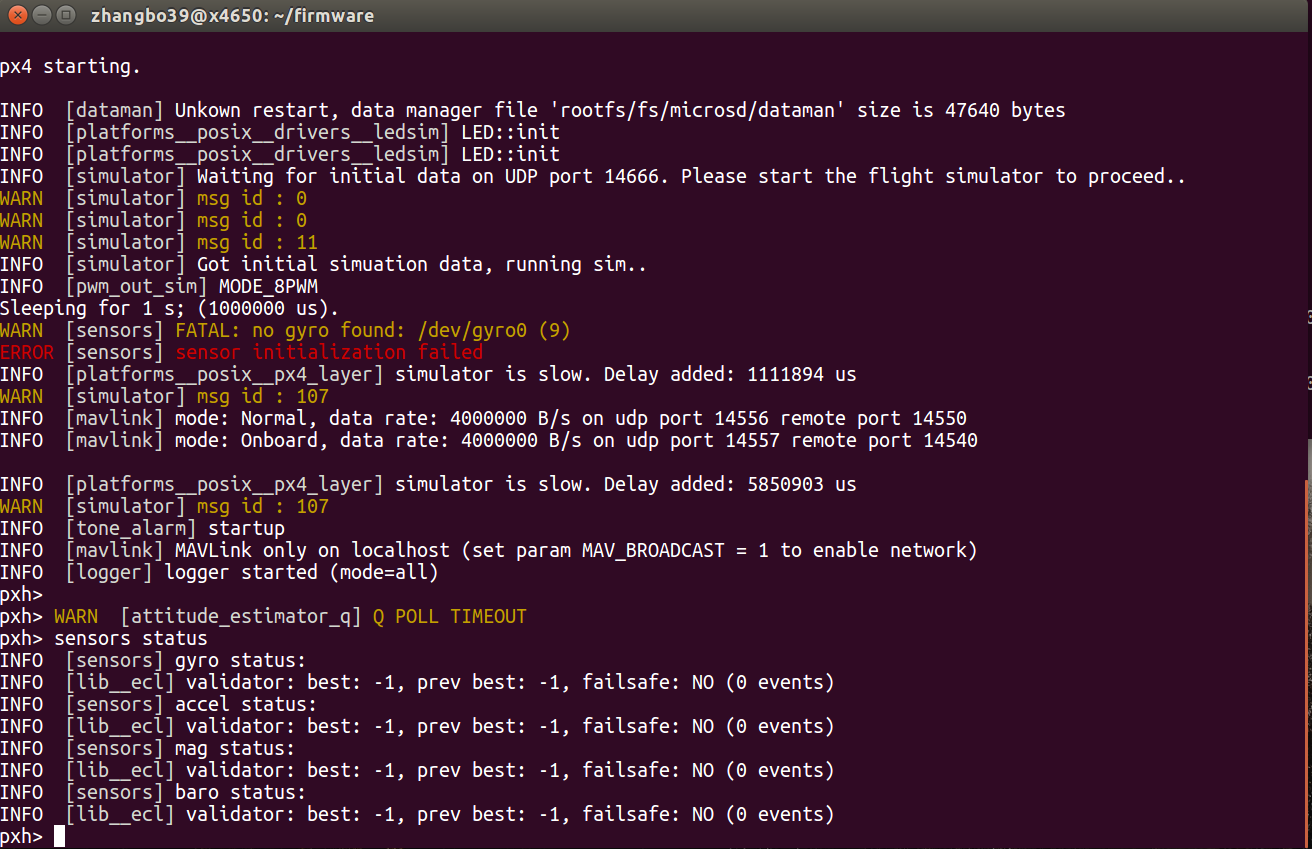
\includegraphics[width = \textwidth,trim = 0 -0 0 -0,clip]{sensors01.png}	  
	\caption{\label{fig: 1} 阻塞等待gyro数据时屏蔽gyrosim}
\end{figure}

\begin{figure}[htbp]
	\figskip
	\centering
	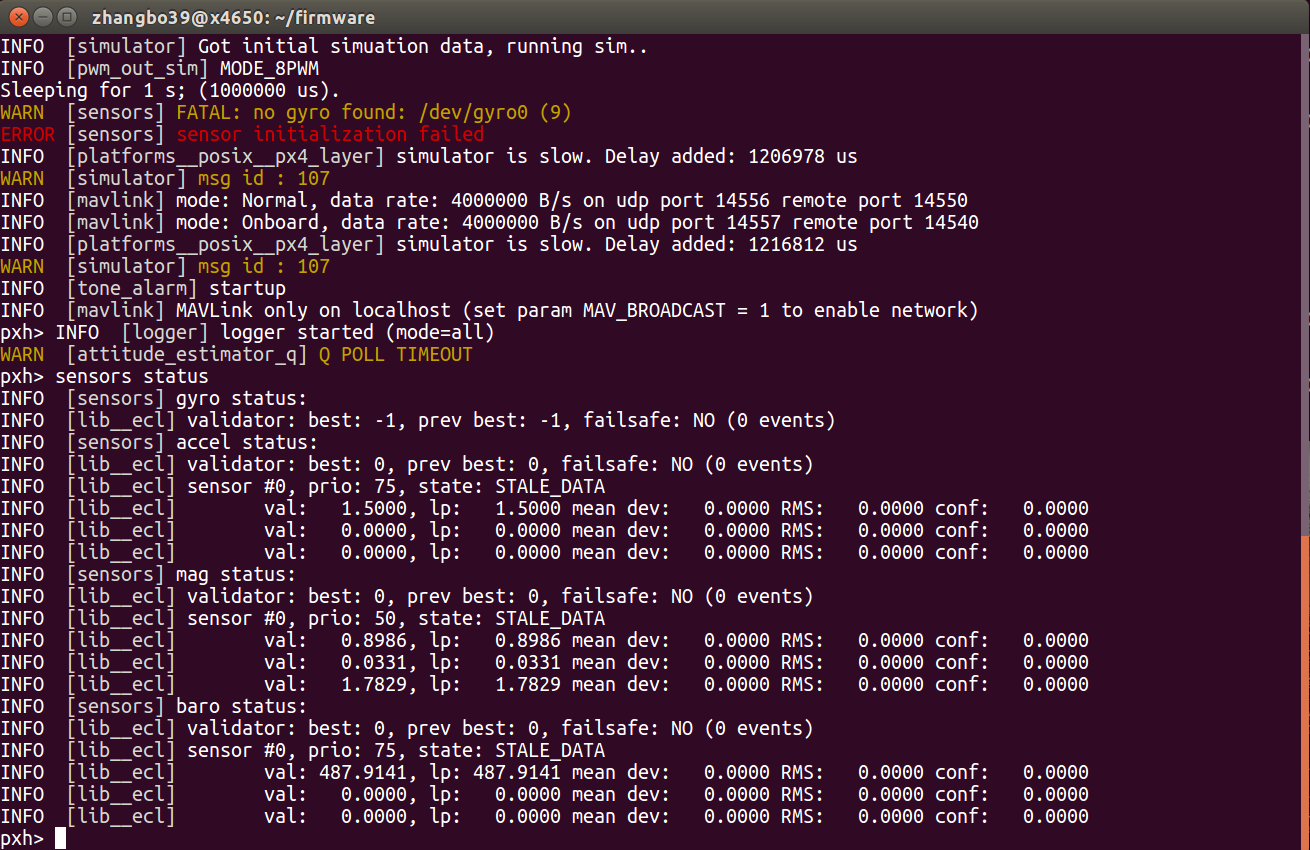
\includegraphics[width = \textwidth,trim = 0 -0 0 -0,clip]{sensors02.png}	  
	\caption{\label{fig: 2} 阻塞等待accel数据时屏蔽gyrosim}
\end{figure}

\subsubsection{pwm_out_sim与mixer模块流程}
\texttt{pwm_out_sim} 的主体PWMSIM类继承自虚拟设备类,包含有一个设备io接口。
\begin{lstlisting}[language=c++,numbers=left,firstnumber = 1,breaklines = true,numberstyle=\tiny,keywordstyle=\color{blue!70},commentstyle=\color{red!50!green!50!blue!50},frame=shadowbox, rulesepcolor=\color{red!20!green!20!blue!20}]
#ifdef __PX4_NUTTX
class PWMSim : public device::CDev
#else
class PWMSim : public device::VDev
#endif
{
public:
...
virtual int     ioctl(device::file_t *filp, int cmd, unsigned long arg);
\end{lstlisting}
在PWMSIM构造函数中,就将\texttt{pwm_out_sim}的设备地址绑定为\texttt{"/dev/pwm_output0"}(宏定义变量为PWM_OUTPUT0_DEVICE_PATH),因此在mixer中load后的地址也是指向这个设备,从而在mixer的load函数中,进行MIXERIOCRESET、MIXERIOCLOADBUF两个指令时都是调用了\texttt{PWMSim::ioctl()}函数。通过这个load函数完成了混控器的初始化(构造混控列表等)。

\texttt{pwm_out_sim}的基本流程就是先设置模式,包含输出通道数量(4)、通信频率(50Hz)等。随后再启动\texttt{PWMSim::task_main_trampoline}线程,负责订阅控制器的控制量,经过混控后再发布出去。

\subsubsection{MAVLink 解析}

SIL中UDP发送与接收的数据都是按照 MAVLink 协议打包的。对于PX4端向UDP发送数据,调用的是\texttt{simulator_mavlink.cpp}中的函数
\begin{lstlisting}[language=c++,numbers=left,firstnumber = 1,breaklines = true,numberstyle=\tiny,keywordstyle=\color{blue!70},commentstyle=\color{red!50!green!50!blue!50},frame=shadowbox, rulesepcolor=\color{red!20!green!20!blue!20}]
	void Simulator::send_mavlink_message(const uint8_t msgid, const void *msg, uint8_t component_ID)
\end{lstlisting}

而对于从UDP取数据到PX4,调用的入口是\texttt{mavlink_parse_char()}函数,这些函数与HIL/真实飞行模式是共用的,因此在SIL中的接收数据并解包的过程与常规模式相同。

另外,如果在常规模式中修改了通信协议,那么SIL中共需要修改两个地方,一个是发送的部分(即\texttt{Simulator::send_mavlink_message()}函数),另一个是将\texttt{simulator.h}中包含的头文件修改与常规模式一致。

\subsubsection{其他 MAVLink 问题}
1. Payload中每个字段都使用小端模式,低位在前、高位在后。

2. Payload中字段的顺序是按照每个字段type size降序排列的,若有拓展字段,则在排序后追加。

3. CRC校验中,包头FE并不校验,在包尾还会增加两个额为校验位(extraCRC),该校验位的计算与每一条消息的消息名称、payload中字段类型、字段名、字段数组长度等计算。心跳包计算结果为50,所以增加的校验位为'0x32'。具体的计算方法可以参考jMAVSim,或者可以参考mavlink库中的宏定义\texttt{MAVLINK_MESSAGE_CRCS}。需要注意的是该宏定义的实现在 mavlink1.0 和 mavlink2.0 是不同的。

\subsection{仿真通信流程}
在基本的仿真准备完成后,一个相对完整的仿真通信流程是这样的:

1. hilSystem会按照固定的时间间隔(1000ms)向端口14560发心跳包,msgID=0。SIM-->PX4

2. autopilotMAVLinkPort监听到 PX4-->SIM 的心跳包,转发给hilSystem做收到心跳后的第一次处理。

3. 当hilSystem第二次收到 PX4-->SIM 的心跳包后,初始化MAVLink:向PX4发送msgID=11的消息,标示出自己的sysID,并将PX4置为 disarmed。此时初始化完成,在hilSystem发送心跳的过程时,也会发送仿真系统状态,分别用107、115、113号消息。

4. PX4-->SIM 发送76号消息,其中指令为511(设置消息间隔),param1=115(指定为115号消息,HIL_STATE_QUATERNION),param2=5000(该消息间隔为5000us)。

5. PX4-->SIM 按照一定的间隔发送93号消息,即飞控算出的各个电机输出值。按照MAVLink协议,\#93消息中的控制量取值-1 .. 1, 然而在PX4源码和jMAVSim中,都将该值视为{\color{red} 0 .. 1之间的值}。jMAVSim端见\texttt{Rotor.java}文件,PX4源码见\texttt{simulator_mavlink.cpp}中的函数:
\begin{lstlisting}[language=c++,numbers=left,firstnumber = 1,breaklines = true,numberstyle=\tiny,keywordstyle=\color{blue!70},commentstyle=\color{red!50!green!50!blue!50},frame=shadowbox, rulesepcolor=\color{red!20!green!20!blue!20}]
void Simulator::pack_actuator_message(mavlink_hil_actuator_controls_t &msg, unsigned index);
\end{lstlisting}

\subsection{Simulink与PX4进行SIL仿真}



\section{硬件在环仿真HIL}
\subsection{启动流程}
jMAVSim在HIL模式下启动指令为:
\begin{lstlisting}[language=sh,numbers=left,firstnumber = 1,breaklines = true,numberstyle=\tiny,keywordstyle=\color{blue!70},commentstyle=\color{red!50!green!50!blue!50},frame=shadowbox, rulesepcolor=\color{red!20!green!20!blue!20}]
java -Djava.ext.dirs= -cp lib/*:out/production/jmavsim.jar me.drton.jmavsim.Simulator -serial /dev/ttyACM0 921600 -qgc
\end{lstlisting}

PX4 在HIL模式下,使用的固件仍然是正常飞行时的px4fmu-v2_default这个,变化的地方在于机型选择,需要使用仿真机型:
\begin{figure}[htbp]
	\figskip
	\centering
	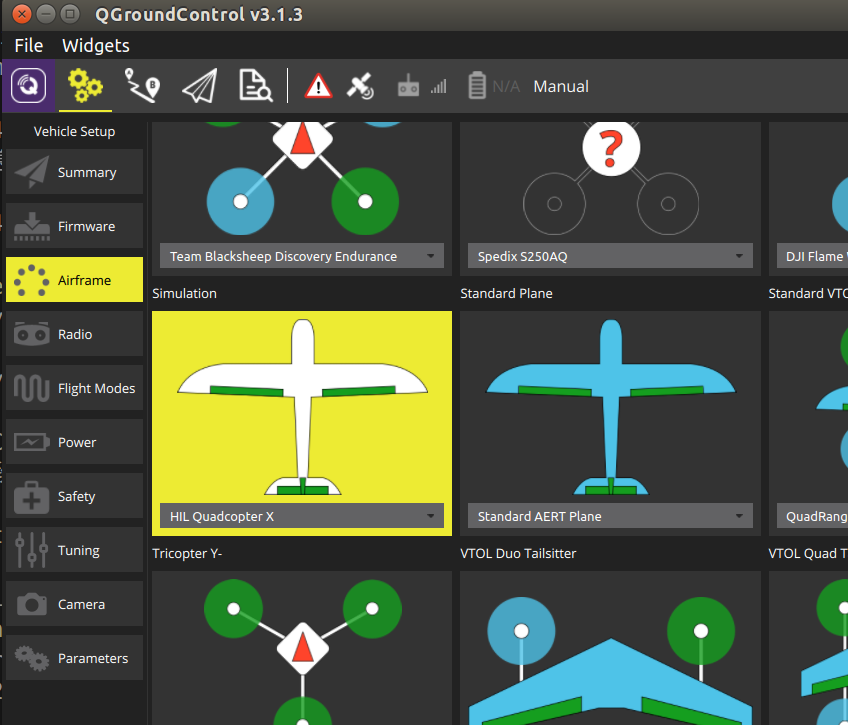
\includegraphics[width = 0.5\textwidth,trim = 0 -0 0 -0,clip]{HIL-2.png}	  
	\caption{\label{fig: HIL2} HIL模式时需要选择的机型}
\end{figure}
对应的系统参数应该是\texttt{SYS_AUTOSTART},选择HIL Quadcopter X时对应于1001:
\begin{figure}[htbp]
	\begin{minipage}[t]{0.5\textwidth}
	\centering
	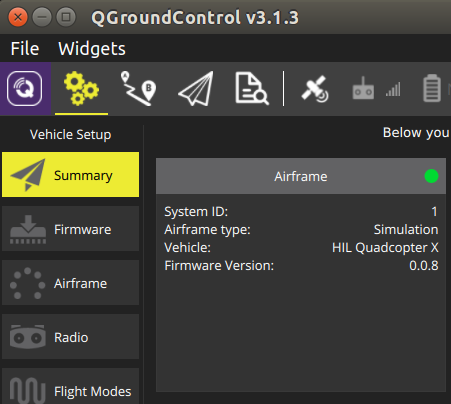
\includegraphics[width = 0.8\textwidth]{HIL-1.png}
	\caption{\label{fig:HIL1}HIL模式下的机型}
	\end{minipage}
	\begin{minipage}[t]{0.5\textwidth}
	\centering
	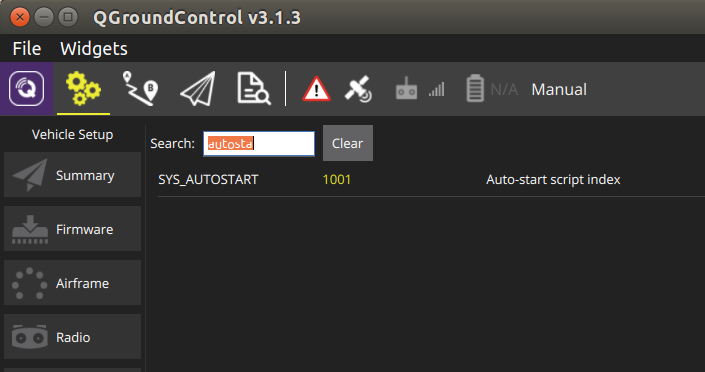
\includegraphics[width = 0.95\textwidth]{HIL-3.png}
	\caption{\label{fig:HIL3}HIL模式下对应的参数}
	\end{minipage}
\end{figure}

HIL在初始化时的启动文件也是\texttt{/firmware/ROMFS/px4fmu_common/init.d/rcS},其中会调用编译时生成的\texttt{/etc/init.d/rc.autostart}的文件。在这个rc.autostart文件中,通过比较\texttt{SYS_AUTOSTART}来确定执行\texttt{/etc/init.d/}文件夹下的机型脚本。1001对应于1001_rc_quad_x.hil,内容为:
\begin{lstlisting}[language=sh,numbers=left,firstnumber = 1,breaklines = true,numberstyle=\tiny,keywordstyle=\color{blue!70},commentstyle=\color{red!50!green!50!blue!50},frame=shadowbox, rulesepcolor=\color{red!20!green!20!blue!20}]
	#!nsh 
	#
	# @name HIL Quadcopter X
	#
	# @type Simulation
	#
	# @maintainer Anton Babushkin <anton@px4.io>
	#
	
	sh /etc/init.d/rc.mc_defaults
	
	set MIXER quad_x
	
	set HIL yes
\end{lstlisting}
主要参数是将\texttt{HIL}变量置为\texttt{yes},这个变量在rcS中的作用:(1)commander的启动方式为\texttt{"commander start -hil"};(2)启动\texttt{pwm_out_sim},且参数为\texttt{mode_pwm16}。pwm_out_sim的启动及其参数与SIL中的作用基本一致。commander采用hil模式时,会在线程中设置变量\texttt{startup_in_hil}
\begin{lstlisting}[language=C++,numbers=left,firstnumber = 0,breaklines = true,numberstyle=\tiny,keywordstyle=\color{blue!70},commentstyle=\color{red!50!green!50!blue!50},frame=shadowbox, rulesepcolor=\color{red!20!green!20!blue!20}]
	if (argc > 2) {
		if (!strcmp(argv[2],"-hil")) {
			startup_in_hil = true;
		} else {
			PX4_ERR("Argument %s not supported, abort.", argv[2]);
			thread_should_exit = true;
		}
	}
\end{lstlisting}
接着设置变量\texttt{status.hil_state}
\begin{lstlisting}[language=C++,numbers=left,firstnumber = 0,breaklines = true,numberstyle=\tiny,keywordstyle=\color{blue!70},commentstyle=\color{red!50!green!50!blue!50},frame=shadowbox, rulesepcolor=\color{red!20!green!20!blue!20}]
	if (startup_in_hil) {
		status.hil_state = vehicle_status_s::HIL_STATE_ON;
	} else {
		status.hil_state = vehicle_status_s::HIL_STATE_OFF;
	}
\end{lstlisting}
并在函数\texttt{set_control_mode}中:
\begin{lstlisting}[language=C++,numbers=left,firstnumber = 0,breaklines = true,numberstyle=\tiny,keywordstyle=\color{blue!70},commentstyle=\color{red!50!green!50!blue!50},frame=shadowbox, rulesepcolor=\color{red!20!green!20!blue!20}]
	control_mode.flag_system_hil_enabled = status.hil_state == vehicle_status_s::HIL_STATE_ON;
\end{lstlisting}
同时也会发布出去:
\begin{lstlisting}[language=C++,numbers=left,firstnumber = 0,breaklines = true,numberstyle=\tiny,keywordstyle=\color{blue!70},commentstyle=\color{red!50!green!50!blue!50},frame=shadowbox, rulesepcolor=\color{red!20!green!20!blue!20}]
	if (counter % (200000 / COMMANDER_MONITORING_INTERVAL) == 0 || status_changed) {
		set_control_mode();
		control_mode.timestamp = now;
		orb_publish(ORB_ID(vehicle_control_mode), control_mode_pub, &control_mode);
\end{lstlisting}
这个\texttt{vehicle_control_mode}会在sensors.cpp中的vehicle_control_mode_poll()函数中被订阅:
\begin{lstlisting}[language=C++,numbers=left,firstnumber = 1,breaklines = true,numberstyle=\tiny,keywordstyle=\color{blue!70},commentstyle=\color{red!50!green!50!blue!50},frame=shadowbox, rulesepcolor=\color{red!20!green!20!blue!20}]
void Sensors::vehicle_control_mode_poll()
{
	struct vehicle_control_mode_s vcontrol_mode;
	bool vcontrol_mode_updated;

	/* Check HIL state if vehicle control mode has changed */
	orb_check(_vcontrol_mode_sub, &vcontrol_mode_updated);

	if (vcontrol_mode_updated) {

		orb_copy(ORB_ID(vehicle_control_mode), _vcontrol_mode_sub, &vcontrol_mode);
		_armed = vcontrol_mode.flag_armed;

		/* switching from non-HIL to HIL mode */
		if (vcontrol_mode.flag_system_hil_enabled && !_hil_enabled) {
			_hil_enabled = true;
			_publishing = false;
			/* switching from HIL to non-HIL mode */

		} else if (!_publishing && !_hil_enabled) {
			_hil_enabled = false;
			_publishing = true;
		}
	}
}
\end{lstlisting}
其作用就是给变量\texttt{_publishing}赋值,而这个值在\texttt{Sensors::task_main()}中会决定是否将sensors中综合得到的传感器数据发布除去:
\begin{lstlisting}[language=C++,numbers=left,firstnumber = 1,breaklines = true,numberstyle=\tiny,keywordstyle=\color{blue!70},commentstyle=\color{red!50!green!50!blue!50},frame=shadowbox, rulesepcolor=\color{red!20!green!20!blue!20}]
if (_publishing && raw.timestamp > 0) {
	
				/* construct relative timestamps */
				if (_last_accel_timestamp[_accel.last_best_vote]) {
					raw.accelerometer_timestamp_relative = (int32_t)(_last_accel_timestamp[_accel.last_best_vote] - raw.timestamp);
				}
	
				if (_last_mag_timestamp[_mag.last_best_vote]) {
					raw.magnetometer_timestamp_relative = (int32_t)(_last_mag_timestamp[_mag.last_best_vote] - raw.timestamp);
				}
	
				if (_last_baro_timestamp[_baro.last_best_vote]) {
					raw.baro_timestamp_relative = (int32_t)(_last_baro_timestamp[_baro.last_best_vote] - raw.timestamp);
				}
	
				orb_publish(ORB_ID(sensor_combined), _sensor_pub, &raw);
\end{lstlisting}
综合来看,如果是HIL模式,sensors中的传感器数据不会发布到\texttt{sensor_combined}这个topic上,导航模块中订阅的传感器信息也就不是sensors发出的了。

实际在HIL模式中,从串口获取仿真数据并发布给导航的流程为:rcS启动串口的mavlink之后,也会订阅\texttt{vehicle_control_mode}这个topic,并设置\texttt{_hil_enabled = true},这样当\texttt{MavlinkReceiver::handle_message()}函数收到msg后,会在解析hil消息后并进行发布。在\texttt{MavlinkReceiver::handle_message_hil_sensor()}函数中,会将数据发布到\texttt{sensor_gyro}等传感器数据以及\texttt{sensor_combined}这个导航使用的topic中。

而在HIL模式中,将飞控数据用mavlink协议从串口发送的流程为:mavlink 启动后会生成一个MavLinkStream链表,在mavlink_main.cpp中的\texttt{int Mavlink::task_main()}函数中,会执行:
\begin{lstlisting}[language=C++,numbers=left,firstnumber = 1,breaklines = true,numberstyle=\tiny,keywordstyle=\color{blue!70},commentstyle=\color{red!50!green!50!blue!50},frame=shadowbox, rulesepcolor=\color{red!20!green!20!blue!20}]
/* update streams */
MavlinkStream *stream;
LL_FOREACH(_streams, stream) {
	stream->update(t);
}
\end{lstlisting}
这样就会在链表中调用每一个stream节点的update()成员函数。在update()函数中,会判断当前时间是否超过了上次发送后的间隔,然后调用send(t)进行数据发送。

综合来看,在HIL模式下数据的接收与发送都是通过mavlink相关的模块来实现的,而SIL中则是用simulator实现数据中转的。

另外要注意的是,虽然sensors不发布\texttt{sensor_combined}这个topic,但是sensors以及其他的传感器模块(mpu6000等)的线程仍然在进行,所以传感器数据(HIL时飞控板的真实传感器数据)仍然会读取并在sensors中订阅,所以如果在nsh中用\texttt{sensors status}命令查看状态,依然会出现多个传感器的数据:
\begin{figure}[htbp]
	\figskip
	\centering
	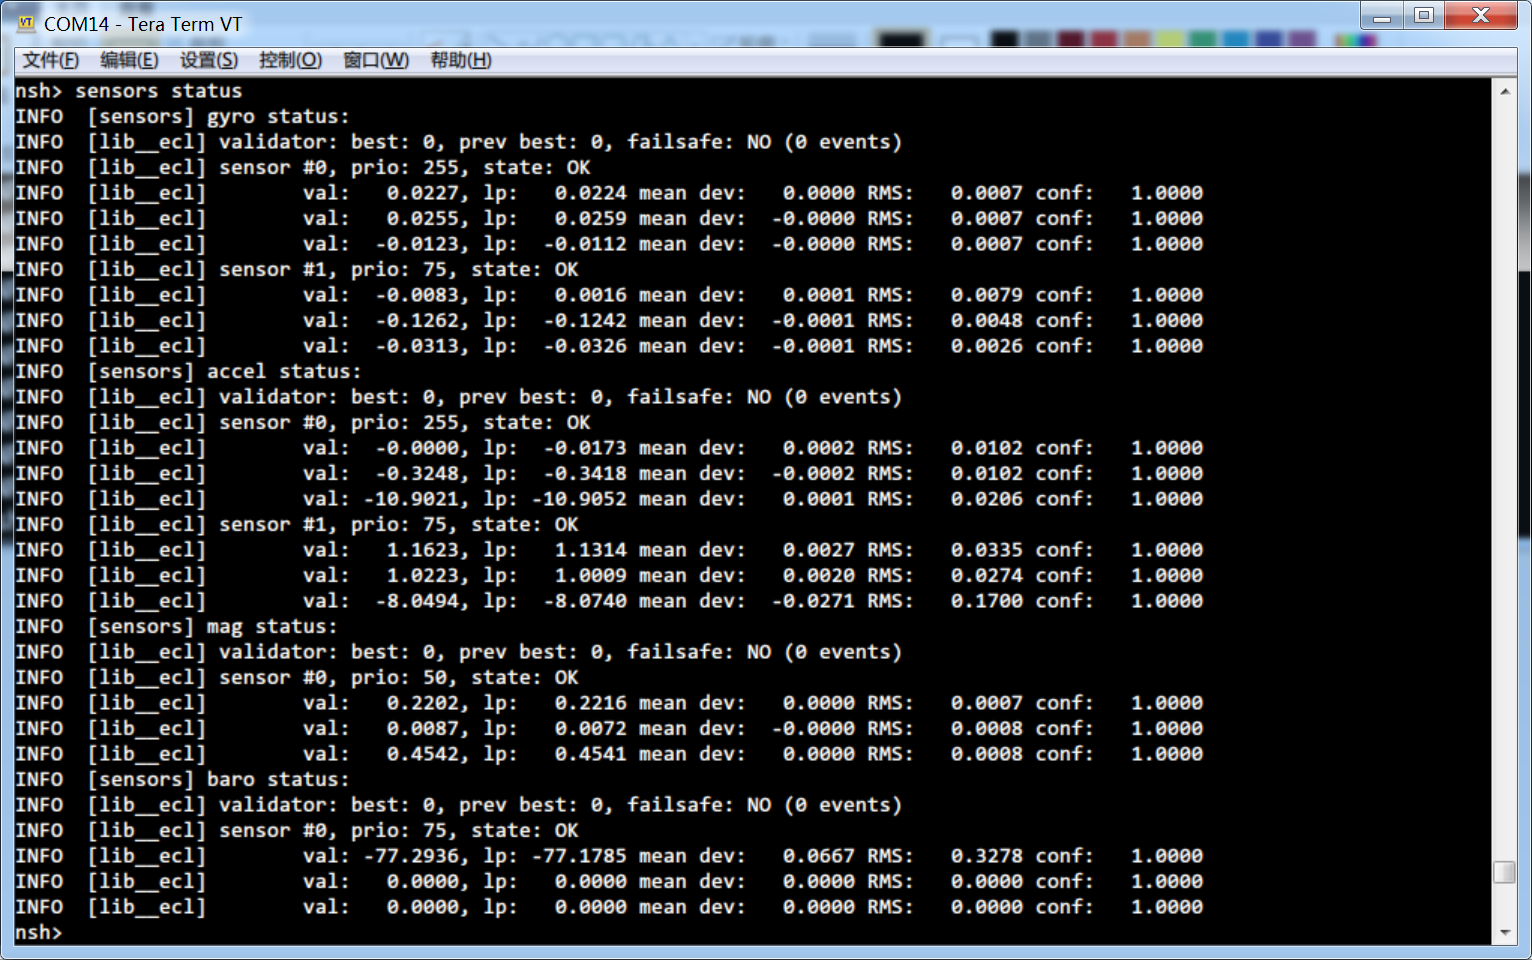
\includegraphics[width = 0.75\textwidth,trim = 0 -0 0 -0,clip]{nsh-0.png}	  
	\caption{\label{fig: sensors0} HIL模式下飞控通电,未连接jMAVSim时的sensors status}
\end{figure}

\begin{figure}[htbp]
	\figskip
	\centering
	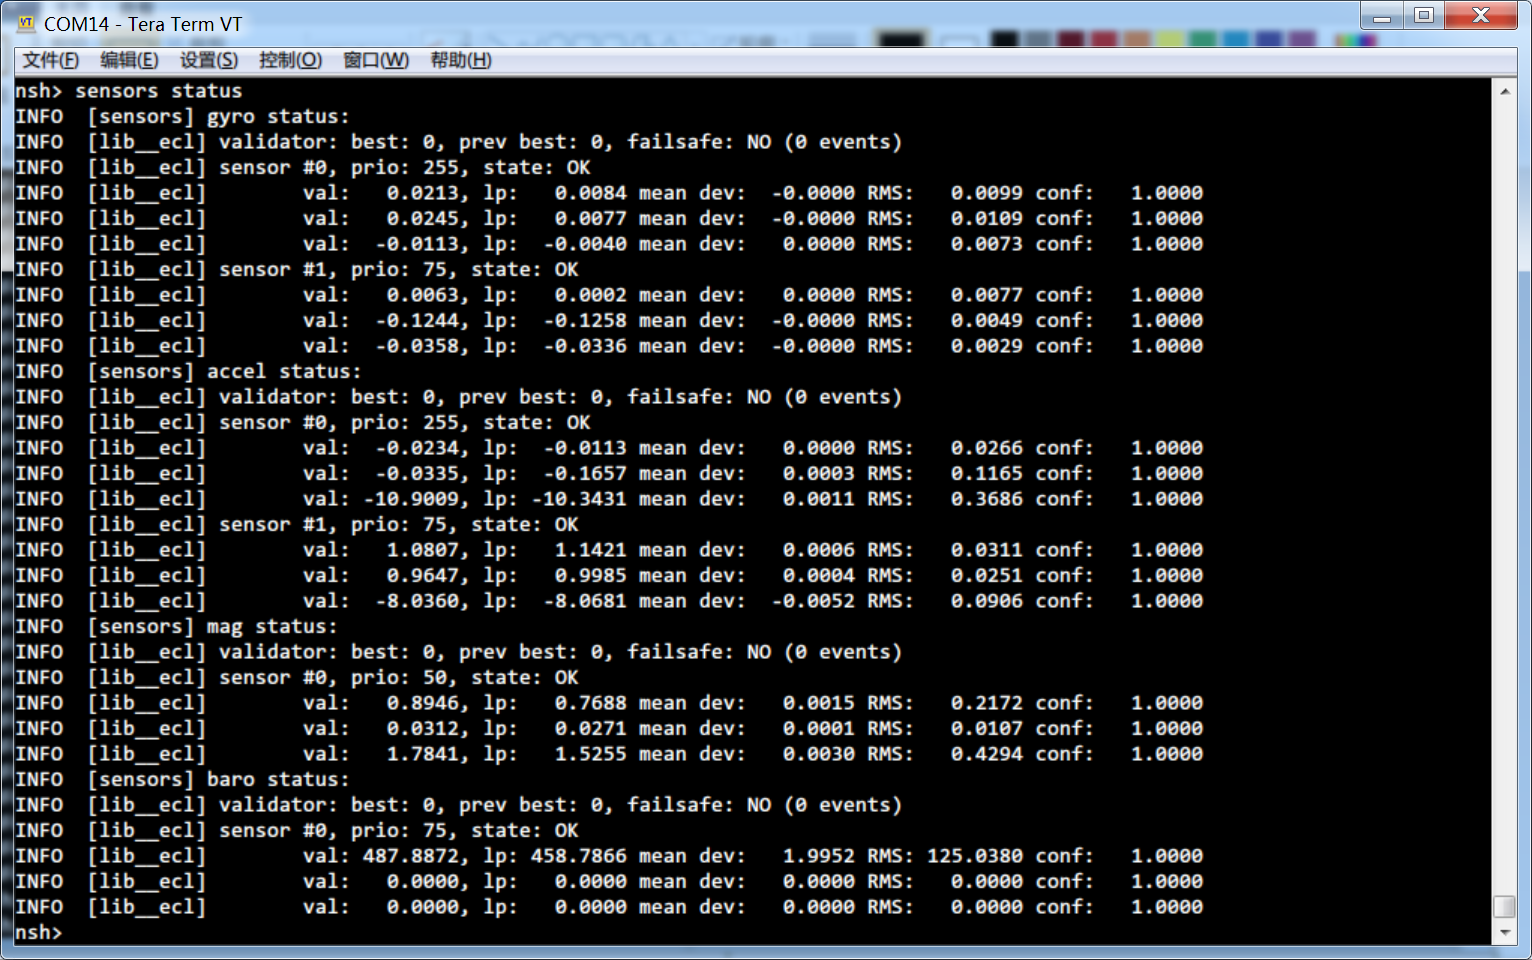
\includegraphics[width = 0.75\textwidth,trim = 0 -0 0 -0,clip]{nsh-0-hil.png}	  
	\caption{\label{fig: sensors1} HIL模式下飞控通电,连接jMAVSim之后的sensors status}
\end{figure}
从上面的图\ref{fig: sensors0}和图\ref{fig: sensors1}可知,确实能够读到多个传感器数据,并且连接jMAVSim之后默认的传感器数据都是仿真数据。而\texttt{baro}气压计状态更清晰的说明,未连接jMAVSim或jMAVSim没发数据的时候,\texttt{sensors status}的读数是飞控的真实数据。

进一步分析可知,由于真实传感器以及MavlinkReceiver中发布数据都是按照单传感器模式(\texttt{orb_advertise()}, 则优先级为默认值75)发布,所以两者的数据会发生重叠,这样即使真实气压计和jMAVSim都有baro数据,但\texttt{sensors status}中baro只有一个数据。所以如果在\texttt{void MavlinkReceiver::handle_message_hil_sensor(mavlink_message_t *msg)}函数中使用\texttt{orb_advertise_multi()}进行声明优先级为100(\texttt{ORB_PRIO_HIGH}),就能够显示多个baro数据了:
\begin{lstlisting}[language=C++,numbers=left,firstnumber = 1,breaklines = true,numberstyle=\tiny,keywordstyle=\color{blue!70},commentstyle=\color{red!50!green!50!blue!50},frame=shadowbox, rulesepcolor=\color{red!20!green!20!blue!20}]
	/* baro */
	{
		struct baro_report baro = {};

		baro.timestamp = timestamp;
		baro.pressure = imu.abs_pressure;
		baro.altitude = imu.pressure_alt;
		baro.temperature = imu.temperature;
		int a = -1;
		if (_baro_pub == nullptr) {
			// _baro_pub = orb_advertise(ORB_ID(sensor_baro), &baro);
			_baro_pub = orb_advertise_multi(ORB_ID(sensor_baro), &baro, &a, ORB_PRIO_HIGH);

		} else {
			orb_publish(ORB_ID(sensor_baro), _baro_pub, &baro);
		}
	}
\end{lstlisting}

\begin{figure}[htbp]
	\figskip
	\centering
	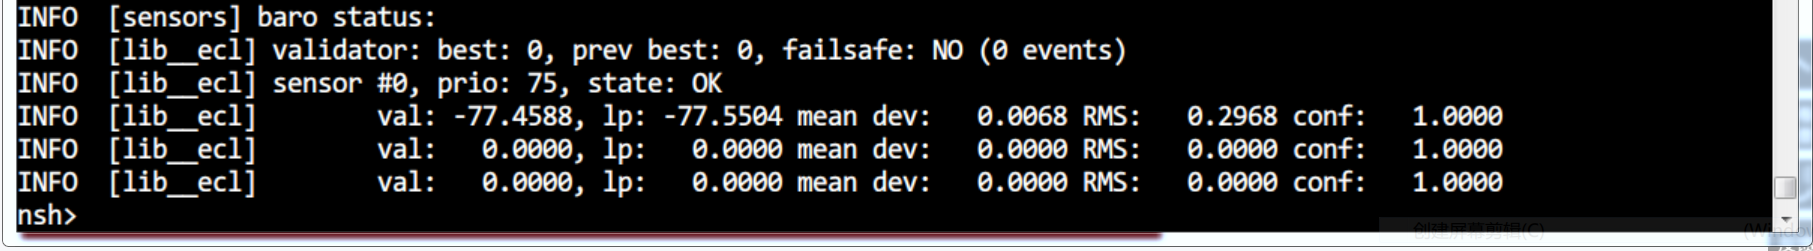
\includegraphics[width = 0.9\textwidth,trim = 0 -0 0 -0,clip]{nsh-1.png}	  
	\caption{\label{fig: sensors2} HIL模式下飞控通电,未连接jMAVSim时的baro}
\end{figure}

\begin{figure}[htbp]
	\figskip
	\centering
	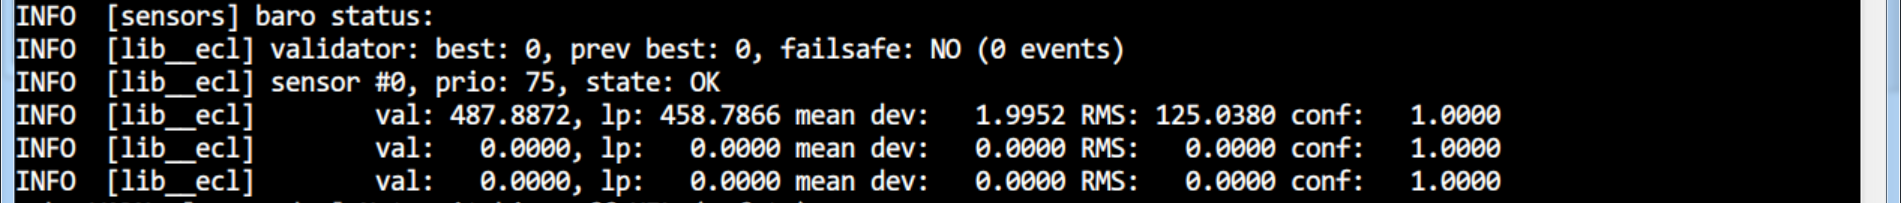
\includegraphics[width = 0.9\textwidth,trim = 0 -0 0 -0,clip]{nsh-2.png}	  
	\caption{\label{fig: sensors3} HIL模式下飞控通电,连接jMAVSim之后的baro}
\end{figure}

\begin{figure}[htbp]
	\figskip 
	\centering
	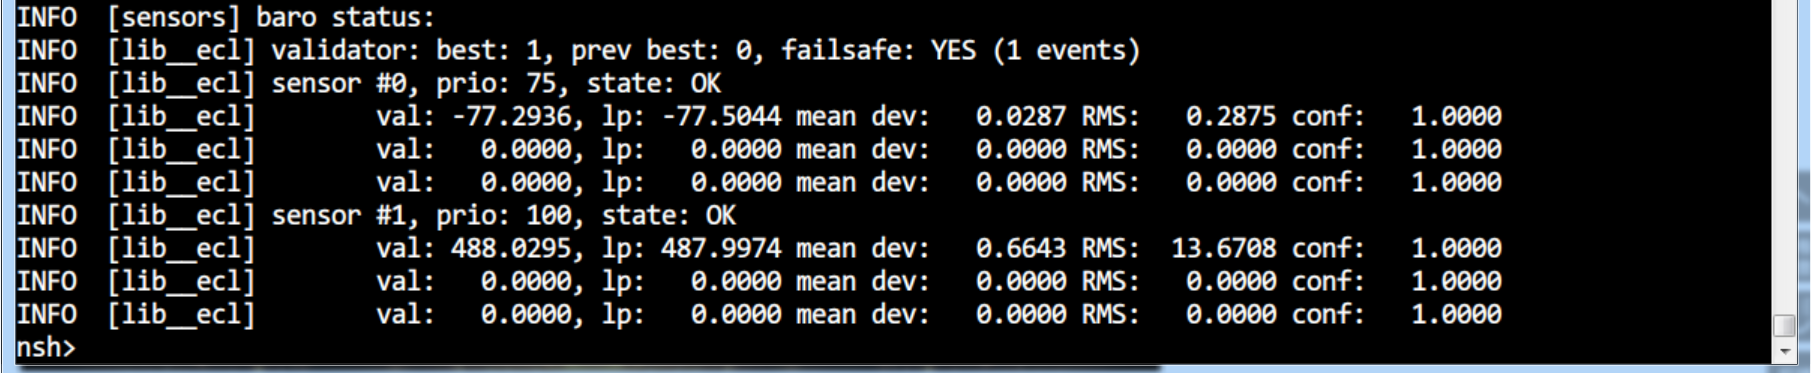
\includegraphics[width = 0.9\textwidth,trim = 0 -0 0 -0,clip]{nsh-3.png}	  
	\caption{\label{fig: sensors4} 增加优先级后,连接jMAVSim之后的baro}
\end{figure}

\subsection{jMAVSim启动时间的讨论}
虽然\href{http://www.pixhawk.com/dev/hil/jmavsim#hardware_in_the_loop_hitl}{官网教程}中介绍了HIL模式的连接方式,但是对于飞控上电和jMAVSim开启的先后并没有说明。按照字面正常推断,应该是飞控首先上电,然后在PC端打开jMAVSim软件(如果先开启jMAVSim的话,由于串口没有数据通信,jMAVSim会自动关闭)。

这里就存在一个飞控上电与jMAVSim启动间隔时间的问题。经过测试,采用INAV导航算法时,如果在一定时间之后才启动jMAVSim(向PX4发送数据)的话,飞控将不能锁定HOME点坐标。对应的现象是能够获取初始GPS,但无法定位当前飞控坐标,也无法响应mission等指令。原因如下:

在\texttt{position_estimator_inav_main.cpp}中,飞控上电后会启动导航主线程\texttt{position_estimator_inav_thread_main}。与其他的常规主线程类似,在阻塞等待数据更新这个主循环之前,是对导航状态量的初始化过程。而这个初始化流程的最后一步是等待并采集一定数量的气压高数据,最后确定气压高偏移值,并将\texttt{local_pos.z_valid} 置为真。那如果jMAVSim一直为发送气压数据,经过一定的等待时间(\texttt{MAX_WAIT_FOR_BARO_SAMPLE=3s})后,也会结束等待气压数据,而这时\texttt{local_pos.z_valid}仍为假。具体代码如下。
\begin{lstlisting}[language=C++,numbers=left,firstnumber = 1,breaklines = true,numberstyle=\tiny,keywordstyle=\color{blue!70},commentstyle=\color{red!50!green!50!blue!50},frame=shadowbox, rulesepcolor=\color{red!20!green!20!blue!20}]
while (wait_baro && !thread_should_exit) {
	int ret = px4_poll(&fds_init[0], 1, 1000);

	if (ret < 0) {
		/* poll error */
		mavlink_log_info(&mavlink_log_pub, "[inav] poll error on init");

	} else if (hrt_absolute_time() - baro_wait_for_sample_time > MAX_WAIT_FOR_BARO_SAMPLE) {
		wait_baro = false;
		mavlink_log_info(&mavlink_log_pub, "[inav] timed out waiting for a baro sample");

	} else if (ret > 0) {
		if (fds_init[0].revents & POLLIN) {
			orb_copy(ORB_ID(sensor_combined), sensor_combined_sub, &sensor);

			if (wait_baro && sensor.timestamp + sensor.baro_timestamp_relative != baro_timestamp) {
				baro_timestamp = sensor.timestamp + sensor.baro_timestamp_relative;
				baro_wait_for_sample_time = hrt_absolute_time();

				/* mean calculation over several measurements */
				if (baro_init_cnt < baro_init_num) {
					if (PX4_ISFINITE(sensor.baro_alt_meter)) {
						baro_offset += sensor.baro_alt_meter;
						baro_init_cnt++;
					}

				} else {
					wait_baro = false;
					baro_offset /= (float) baro_init_cnt;
					local_pos.z_valid = true;
					local_pos.v_z_valid = true;
				}
			}
		}

	} else {
		PX4_WARN("INAV poll timeout");
	}
}
\end{lstlisting}

最后发布\texttt{vehicle_global_position}消息时的判别条件是\texttt{if (local_pos.xy_global \&\& local_pos.z_global)}。显然jMAVSim启动时间会影响到这里的消息发布。所以即便之后飞控收到了GPS数据,但\texttt{vehicle_global_position}也始终无法发布,之后也就会遇到前文中出现的现象了。



% \begin{lstlisting}[language=C++,numbers=left,firstnumber = 0,breaklines = true,numberstyle=\tiny,keywordstyle=\color{blue!70},commentstyle=\color{red!50!green!50!blue!50},frame=shadowbox, rulesepcolor=\color{red!20!green!20!blue!20}]
% \end{lstlisting}





















\cleardoublepage

\chapter{ROS}
\section{基础}
\subsection{创建工作空间}
\begin{lstlisting}[language=bash,numbers=left,firstnumber = 1,numberstyle=\tiny,breaklines = true,keywordstyle=\color{blue!70},commentstyle=\color{red!50!green!50!blue!50},frame=shadowbox, rulesepcolor=\color{red!20!green!20!blue!20}]
mkdir -p ~/workspace/src
cd ~/workspace
catkin_make
source devel/setup.bash
\end{lstlisting}

\subsection{创建一个pkg}
\begin{lstlisting}[language=bash,numbers=left,firstnumber = 1,numberstyle=\tiny,breaklines = true,keywordstyle=\color{blue!70},commentstyle=\color{red!50!green!50!blue!50},frame=shadowbox, rulesepcolor=\color{red!20!green!20!blue!20}]
cd ~/workspace/src
catkin_create_pkg pkgname std_msgs rospy roscpp
cd ~/workspace
catkin_make
\end{lstlisting}







\subsection{编译git上的pkg}
1. 创建一个空的文件夹作为工作空间目录

2. git clone 待使用的目标package

3. 在工作空间目录下,使用\texttt{catkin_make --source pkgname}进行编译

4. (似乎可以忽略)使用\texttt{catkin_make install --source pkgname}安装。

5. 使用\texttt{source devel/setup.bash}读取当前工作空间的环境变量。




\subsection{问题及解决方案}
编译报错:ModuleNotFoundError: No module named 'em'
使用 "~\$ pip install em"
编译继续报错:AttributeError: module 'em' has no attribute 'Interpreter'
解决:

pip uninstall em
pip install empy
\chapter{Python3 学习使用}
\section{Python3 生成PDF文档}
初始的需求是将测试设备得到的测量数据,自动生成为测试报告。其中测量数据形式为$[\bf{t}, \bf{D}_1, \bf{D}_2, \dots, \bf{D}_n]$这样的数据集,第一列为时间戳,后续为特定数据。考虑到通用性和开发便捷性,以及对数据处理和绘图的要求,考虑采用Python3 生成PDF文档。特别标明用的Py3版本是因为在某些环节中Py2的处理会不适用。

整体流程以及主要使用的包如图\ref{fig: PDF流程}所示:
% 流程图定义基本形状
\tikzstyle{startstop} = [rectangle, rounded corners, minimum width = 2cm, minimum height=1cm,text centered, draw = black, fill = red!40]
\tikzstyle{io} = [trapezium, trapezium left angle=70, trapezium right angle=110, minimum width=2cm, minimum height=1cm, text centered, draw=black, fill = blue!40]
\tikzstyle{process} = [rectangle, minimum width=3cm, minimum height=1cm, text centered, draw=black, fill = yellow!50]
\tikzstyle{decision} = [diamond, aspect = 3, text centered, draw=black, fill = green!30]
% 箭头形式
\tikzstyle{arrow} = [->,>=stealth]

\begin{figure}[htbp]
\centering
\begin{tikzpicture}[node distance=2cm]
%定义流程图具体形状
\node (start) [startstop] {开始};
\node (read) [process, below of=start, yshift = -0.2cm]{读取测试数据};
\node (analysis) [process, below of=read, yshift = -0.2cm]{数据处理及分析};
\node (result) [process, below of=analysis, yshift = -0.2cm]{测试结果及绘图};
\node (getpdf) [process, below of=result, yshift = -0.2cm]{生成PDF文档};
\node (stop) [startstop, below of=getpdf]{结束};

%连接具体形状
\draw [arrow](start) -- (read) ;
\draw [arrow](read) -- node[anchor = west] {NumPy} (analysis);
\draw [arrow](analysis) -- node[anchor = west] {matplotlib} (result);
\draw [arrow](result) -- node[anchor = west] {reportlab} (getpdf);
\draw [arrow](getpdf) -- (stop);
% \draw [arrow](dec1) -- ($(dec1.east) + (1.5,0)$) node[anchor=north] {不通过} |- (pro3);
\end{tikzpicture}
\caption{\label{fig: PDF流程} 自动报告python生成流程}
\end{figure}

\subsection{读取测试数据}
这里默认下位机数据已经回传到上位机中,协议使用csv格式且无第一行变量名称,那么可以直接调用
\begin{lstlisting}[language=python,numbers=left,firstnumber = 1,breaklines = true,numberstyle=\tiny,keywordstyle=\color{blue!70},commentstyle=\color{red!50!green!50!blue!50},frame=shadowbox, rulesepcolor=\color{red!20!green!20!blue!20}]
import numpy, sys
st = sys.argv
if (len(st) > 1):
    filename = st[1].split('.')[0]
else:
    print("Please input log file name!")
    return
data = numpy.loadtxt(open(filename+'.csv',"rb"),delimiter=",",skiprows=0) 
\end{lstlisting}

\subsection{数据分析及处理}
待定

\subsection{测试结果及绘图}
值得注意的是绘图中1维/n维数据的处理、中文处理等。具体代码为:
\begin{lstlisting}[language=python,numbers=left,firstnumber = 1,breaklines = true,numberstyle=\tiny,keywordstyle=\color{blue!70},commentstyle=\color{red!50!green!50!blue!50},frame=shadowbox, rulesepcolor=\color{red!20!green!20!blue!20}]
import matplotlib
import matplotlib.pyplot as plt

#字体路径、尺寸设置
TTFontpath = {'zen':'./wqy-zenhei.ttc','micro':'./wqy-microhei.ttc'}
zhfont2 = matplotlib.font_manager.FontProperties(fname=TTFontpath['micro'])
zhfont1 = matplotlib.font_manager.FontProperties(fname=TTFontpath['zen'])
zhfontlegend = zhfont1
zhfontlegend.set_size(22)

#画图
def getMyImage(x, y, xlabel, ylabel, title, legendstr = ''):
    fig = plt.figure(figsize = (16,16))
    if y.size == y.shape[0]:
        plt.plot(x,y, label = legendstr)
    else:
        for i in range(y.shape[1]):
            plt.plot(x, y[:,i], label = legendstr[i])
    plt.xlabel(xlabel,fontsize = 24, fontproperties=zhfont1)
    plt.ylabel(ylabel,fontsize = 24, fontproperties=zhfont1)
    plt.title(title,fontsize = 28, fontproperties=zhfont1)
    if legendstr != '': 
        plt.legend(loc='best', ncol=y.size//y.shape[0], prop = zhfontlegend, shadow=True, fancybox=True).get_frame().set_alpha(0.4)

#主函数中截选

simt = (data[:,0] - data[0,0]) / 1000.0
curr = data[:,[3,4,7]]
getMyImage(simt, data[:,5], '时间(s)', '温度(度)', '温度曲线')
getMyImage(simt, curr, '时间(s)', '电压(V)', '电调电压曲线',['上电机电调电流','下电机电调电流','总电流'])
\end{lstlisting}
NumPy的array矩阵,如果抽取一列的话,结果是一维向量,这时shape属性的为‘(len,)’,没有第二个值。所以在14行做了特殊的判断。

ubuntu下系统的字体可以在 ‘/usr/share/fonts/truetype/’ 下查找,这里将字体放到项目目录下了。图例中的属性使用‘prop’关键字,而标签、标题则是‘fontsize/fontproperties’等。

\subsection{生成PDF文档}
生成PDF使用reportlab这个包,并且是基于test_charts_textlabels.py这个模板改的。主要的细节有两点,一是中文格式等,二是matplotlib图片怎么直接插入到PDF中(而不用先临时保存为文件)。reportlab包的使用具体可以参考reportlab的手册,或者直接从
\href{https://pypi.python.org/pypi/reportlab/3.4.0}{reportlab3.4源码地址}
下载源码并使用 ‘python3 setup.py install’ 安装,然后生成测试代码、demo、手册等PDF。

中文格式采用以下的办法:
\begin{lstlisting}[language=python,numbers=left,firstnumber = 1,breaklines = true,numberstyle=\tiny,keywordstyle=\color{blue!70},commentstyle=\color{red!50!green!50!blue!50},frame=shadowbox, rulesepcolor=\color{red!20!green!20!blue!20}]
from reportlab.pdfbase import pdfmetrics
from reportlab.pdfbase.ttfonts import TTFont

TTFontpath = {'zen':'./wqy-zenhei.ttc','micro':'./wqy-microhei.ttc'}
pdfmetrics.registerFont(TTFont('micro', TTFontpath['micro']))
pdfmetrics.registerFont(TTFont('zen', TTFontpath['zen']))
\end{lstlisting}
在使用时:
\begin{lstlisting}[language=python,numbers=left,firstnumber = 1,breaklines = true,numberstyle=\tiny,keywordstyle=\color{blue!70},commentstyle=\color{red!50!green!50!blue!50},frame=shadowbox, rulesepcolor=\color{red!20!green!20!blue!20}]
story = []
styleSheet = getSampleStyleSheet()
bt = styleSheet['BodyText']
cbt = styleSheet['BodyText']
h1 = styleSheet['Heading1']
ch1 = styleSheet['Heading1']

cbt.fontName = 'micro'
ch1.fontName ='zen'

story.append(Paragraph('测试标题测试标题', ch1))
story.append(Paragraph('测试文本测试文本', cbt))
\end{lstlisting}

将matplotlib的图片插入到reportlab的PDF中,有2个中间步骤:

(1)将matplotlib的图片对象转为reportlab中的图片对象
\begin{lstlisting}[language=python,numbers=left,firstnumber = 1,breaklines = true,numberstyle=\tiny,keywordstyle=\color{blue!70},commentstyle=\color{red!50!green!50!blue!50},frame=shadowbox, rulesepcolor=\color{red!20!green!20!blue!20}]
#!/usr/bin/env python3
# -*- coding: utf-8 -*-

from PIL import Image
import matplotlib.pyplot as plt
from reportlab.pdfgen import canvas
from reportlab.lib.units import inch, cm

from reportlab.lib.utils import ImageReader

fig = plt.figure(figsize=(4, 3))
plt.plot([1,2,3,4])
plt.ylabel('some numbers')

imgdata = Image.io.BytesIO() #!
fig.savefig(imgdata, format='png')
imgdata.seek(0)  # rewind the data

Image = ImageReader(imgdata) #!

c = canvas.Canvas('test.pdf')
c.drawImage(Image, cm, cm, inch, inch)
c.save()
\end{lstlisting}
以上是能够在Python3中运行的demo,具体参考的是stackoverflow上\href{https://stackoverflow.com/questions/18897511/how-to-drawimage-a-matplotlib-figure-in-a-reportlab-canvas}{How to drawImage a matplotlib figure in a reportlab canvas?}的回答和
\href{https://stackoverflow.com/questions/8598673/how-to-save-a-pylab-figure-into-in-memory-file-which-can-be-read-into-pil-image}{how to save a pylab figure into in-memory file which can be read into PIL image?}的回答。前一个回答中的代码在Python2上没问题,当在Python3中无法使用。

(2)在reportlab的模板中追加图片
\begin{lstlisting}[language=python,numbers=left,firstnumber = 1,breaklines = true,numberstyle=\tiny,keywordstyle=\color{blue!70},commentstyle=\color{red!50!green!50!blue!50},frame=shadowbox, rulesepcolor=\color{red!20!green!20!blue!20}]
class flowable_fig(reportlab.platypus.Flowable):
    def __init__(self, imgdata):
        reportlab.platypus.Flowable.__init__(self)
        self.img = reportlab.lib.utils.ImageReader(imgdata)
    def draw(self):
        self.canv.drawImage(self.img, 0.5 * A4[0]-3.5*inch, 0*inch, height = -3*inch, width = 5*inch)

def getMyImage(x, y, xlabel, ylabel, title, legendstr = ''):
    #...
    imgdata = Image.io.BytesIO()
    fig.savefig(imgdata, format='png')
    imgdata.seek(0)  
    return flowable_fig(imgdata)

#主函数中截选
#...
story.append(getMyImage(simt, data[:,5], '时间(s)', '湿度(%)', '湿度曲线'))
\end{lstlisting}
参考的是\href{https://stackoverflow.com/questions/5356413/draw-images-with-canvas-and-use-simpledoctemplate}{Draw images with canvas and use SimpleDocTemplate}的回答。

\section{数学运算}
16进制与浮点数相互转化:
\begin{lstlisting}[language=python,numbers=left,firstnumber = 1,breaklines = true,numberstyle=\tiny,keywordstyle=\color{blue!70},commentstyle=\color{red!50!green!50!blue!50},frame=shadowbox, rulesepcolor=\color{red!20!green!20!blue!20}]
import struct
struct.unpack('!f', bytes.fromhex('3f660ab9'))[0]
hex(struct.unpack('<I', struct.pack('<f', 2.0000))[0])
\end{lstlisting}


\begin{lstlisting}[title=abcdefg,language=python,numbers=left,firstnumber = 1,breaklines = true,numberstyle=\tiny,keywordstyle=\color{blue!70},commentstyle=\color{red!50!green!50!blue!50},frame=shadowbox, rulesepcolor=\color{red!20!green!20!blue!20}]
    hello world!
\end{lstlisting}


\chapter{状态估计}
\section{基础理论知识}
本节主要参考了文献\texttt{State Estimation for Micro Air Vehicles}的第4、5节内容。
\subsection{低通滤波器}
低通滤波器可以认为是一种较为简单的估计器。常见的一阶低通滤波器可以表示为:
\begin{equation*}
    Y(s) = \frac{a}{s+a}U(s)
\end{equation*}
通过Laplace逆变换可以得到时域形式为:
\begin{equation}
    \dot{y} = -ay+au
\end{equation}
进一步地,求解该微分方程可得:
\begin{equation*}
    y(t+T) = e^{-aT}y(t) + a\int_0^T{e^{-a(T-\tau)}u(\tau)}\dd{\tau}
\end{equation*}
如果用$T_s$表示采样周期,且假设$u(t)$在采样周期内保持常值,那么有:
\begin{align}
    y(k+1) & = e^{-a T_s} y(k) + a \int_0^{T_s}{e^{-a(T_s-\tau)}}\dd{\tau} \cdot u(k) \notag \\
    & = e^{-aT_s} y(k) + (1-e^{-aT_s}) u(k)
\end{align}
定义$\alpha_{LPF} = e ^ {-a T_s}$,则可以进一步简化为:
\begin{equation}
    y(k+1) = \alpha_{LPF} y(k) + (1-\alpha_{LPF}) u(k)
\end{equation}
如果用符号$LPF(\cdot)$表示上述的低通滤波运算,那么$\hat{x} = LPF(x)$就是$x$在低通滤波下的估计值。

\subsection{动态观测器}
考虑一个LTI系统并表示为:
\begin{align*}
    \dot{x} & = A x + B u \\
    y & = C x
\end{align*}
对于该系统的连续时间观测器可以表示为:
\begin{equation}
    \dot{\hat{x}} = A \hat{x} + B u + L(y-C\hat{x})
\end{equation}
其中,$\hat{x}$为$x$的估计值。上式中等号右端前两项可以认为是对原系统的预估,最后一项可以认为是利用观测数据对状态的校正。定义估计误差为$\tilde{x} = x - \hat{x}$,那么可以得到:
\begin{equation}
    \dot{\tilde{x}} = (A - L C)\tilde{x}
\end{equation}
这表明如果选择合适的$L$值使得矩阵$A-LC$是Hurwitz稳定的,那么估计误差将以指数方式收敛到零。

如果观测数据并不是在每一拍都可以获得(传感器数据更新较慢),那么可以采用如下的两步方式进行处理,如图\ref{fig: estimator1}所示。

在没有得到传感器数据的时候,只使用预估方式进行估计:
\begin{equation}
    \dot{\hat{x}} = A \hat{x} + B u    
\end{equation}
当得到传感器数据后,则进行校正:
\begin{equation}
    \hat{x}^+ = \hat{x}^- + L(y(t_k) - C \hat{x}^-)
\end{equation}
其中,$\hat{x}^-$表示预估值,$\hat{x}^+$表示校正值。注意到,在这种处理方式下,并不要求传感器数据以固定频率更新。
\begin{figure}[htbp]
	\figskip
	\centering
	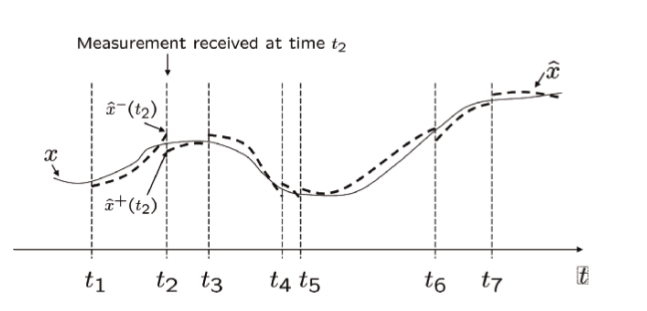
\includegraphics[width = 0.6\textwidth,trim = 0 -0 0 -0,clip]{estimator1.png}	  
	\caption{\label{fig: estimator1} 用动态观测器进行预估-校正方式的状态估计}
\end{figure} 

\subsection{连续--离散卡尔曼滤波器}
考虑如下的系统:
\begin{align}
    \dot{\bm{x}} &= \bm{A} \bm{x} + \bm{B} \bm{u} + \bm{\xi} \notag \\
    \bm{y}_k &= \bm{C} \bm{x}_k + \bm{\eta}_k
\end{align}
其中,状态方程用连续形式表示,观测方程则用离散的形式表示,下标$k$表示第k次采样。
$\bm{\xi}$表示过程噪声,假设均值为0、协方差为$\bf{Q}$,实际中$\bf{Q}$往往是未知的。
$\bm{\eta}_k$表示测量噪声,与传感器特性相关,假设其均值为0、协方差为$\bf{R}$,实际中可以通过传感器标定估计出$\bf{R}$。

那么针对该系统,可以构造与动态观测器形式类似的连续--离散卡尔曼滤波器:
\begin{align}
    \dot{\hat{\bm{x}}} &= \bm{A} \hat{\bm{x}} + \bm{B} \bm{u} \notag \\
    \hat{\bm{x}}^+_k &= \hat{\bm{x}}^-_k + \bm{L} (\bm{y}_k - \bm{C} \hat{\bm{x}}^-_k)
\end{align}

定义滤波器的估计误差$\tilde{\bm{x}} = \bm{x} - \hat{\bm{x}}$,那么估计误差的协方差可以表示为:
\begin{equation}
    \bm{P}(t) = E\left\{ \tilde{\bm{x}}(t) \tilde{\bm{x}}(t)^\uT \right\}
\end{equation}
显然$\bm{P}(t)$是一个对称、半正定的,所以它的特征值均非负。当$\bm{P}(t)$具有较小的特征值时,滤波器估计误差的方差较小,所以这时估计误差也较小。
考虑到
\begin{equation*}
    \rm{tr}(\bm{P}) = \sum{\lambda_i}
\end{equation*} 
{\color{red}所以卡尔曼滤波器就是求解$\bm{L}$使$\rm{tr}(\bm{P})$取得最小值,从而获得在均方误差最小指标下的最优状态估计。}

\noindent {\hei $\blacksquare$ 传感器数据更新前}

对估计误差求导可得:
\begin{align*}
    \dot{\tilde{\bm{x}}} &= \dot{\bm{x}} - \dot{\hat{\bm{x}}} \\
    &= \bm{( Ax+Bu+\xi) - (A\hat{x} + Bu) } \\
    &= \bm{A \tilde{x} + \xi}
\end{align*}
该微分方程的解为:
\begin{equation}
    \bm{\tilde{x}}(t) = e^{\bm{A} t} \tilde{\bm{x}}_0 + \int_0^t{e^{\bm{A} (t-\tau)} \bm{\xi}(\tau)}\dd \tau
\end{equation}
对$\bm{P}$求导可得:
\begin{align*}
    \dot{\bm{P}} &= \D{}{t} E\{\bm{\tilde{x} \tilde{x}^\uT} \} \\
    &= E\{\bm{\dot{\tilde{x}} \tilde{x}^\uT} + \tilde{x}\dot{\tilde{x}}^\uT \} \\
    &= E\{\bm{ A \tilde{x} \tilde{x}^\uT  + \xi\tilde{x}^\uT + \tilde{x}\tilde{x}^\uT A^\uT + \tilde{x} \xi^\uT   } \} \\
    &= \bm{A P + P A^\uT} + E\{ \bm{\xi \tilde{x}^\uT}\} + E\{ \bm{\tilde{x} \xi^\uT} \}
\end{align*}
其中,
\begin{align*}
    E \{ \bm{ \xi \tilde{x}^\uT } \} &= E \left\{ \bm{\xi}(t) \tilde{\bm{x}}_0 e^{\bm{A}^\uT t} 
    + \int_0^t{ \bm{\xi}(t)\bm{\xi}^\uT (\tau) e^{\bm{A}^\uT (t-\tau)} }\dd \tau \right\} \\
    &= \frac 1 2 \bm{Q}
\end{align*}
代入上式可得:
\begin{equation}
    \bm{\dot{P} = A P + P A^\uT + Q}
\end{equation}

\noindent {\hei $\blacksquare$ 传感器数据更新时}

在传感器数据更新时,有:
\begin{equation*}
    \hat{\bm{x}}^+_k = \hat{\bm{x}}^-_k + \bm{L} (\bm{y}_k - \bm{C} \hat{\bm{x}}^-_k)
\end{equation*}
假定$\bm{\eta}$和$\bm{x}$是独立的,也就是$E\{ \tilde{\bm{x}}^- \bm{\eta}^\uT L^\uT  \} = E\{\bm{ L\eta\tilde{x}^{-\uT} }\} = \bm{0}$,那么可以计算$\bm{P}^+$为:
\begin{align}{\label{equ: p+}}
    \bm{P}^+ =& E\{ \tilde{\bm{x}}^+ \tilde{\bm{x}}^{+\uT}   \} \notag \\
            =& E\left\{ \bm{ (\tilde{x}^- - LC\tilde{x}^- - L\eta) (\tilde{x}^- - LC\tilde{x}^- - L\eta)^\uT } \right\}  \notag \\
            =& E\left\{\bm{ \tilde{x}^- \tilde{x}^{-\uT} - \tilde{x}^- \tilde{x}^{-\uT} C^\uT L^\uT - \tilde{x}^- \eta^\uT L^\uT}  \right. \notag \\
            & \bm{ - LC\tilde{x}^- \tilde{x}^{-\uT} + LC \tilde{x}^- \tilde{x}^{-\uT} C^\uT L^\uT + LC\tilde{x}^- \eta^\uT L^\uT}  \notag \\
            & \left. \bm{ - L \eta \tilde{x}^{-\uT} + L \eta \tilde{x}^{-\uT} C^\uT L^\uT + L \eta \eta^\uT L^\uT } \right\}  \notag \\
            =& \bm{ P^- - P^- C^\uT L^\uT - LCP^- + LCP^-C^\uT L^\uT + LRL^\uT }
\end{align}
为了求解使$\rm{tr}(\bm{P}^+)$最小化时的$\bm{L}$值,一个必要的条件为:
\begin{gather*}
    \Q{}{\bm{L}} \rm{tr}(\bm{P}^+) = \bm{-P^- C^\uT - P^- C^\uT + 2LCP^-C^\uT + 2LR} = 0 \\
    \Rightarrow 2 \bm{L(R + CP^-C^\uT)} = 2 \bm{P^-C^\uT} \\
    \Rightarrow \bm{L} = \bm{P^- C^\uT(R+CP^-C^\uT)^{-1}}
\end{gather*}
推导中用到以下矩阵关系:
\begin{gather*}
    \Q{}{\bm{A}} \rm{tr}(\bm{BAD}) = \bm{B^\uT D^\uT} \\
    \Q{}{\bm{A}} \rm{tr}(\bm{ABA^\uT}) = 2 \bm{AB},\,\bm{B} = \bm{B}^\uT
\end{gather*}
将$\bm{L}$的计算式代入式(\ref{equ: p+})中可得:
\begin{equation}
    \bm{P}^+ = \bm{(I - LC)P^-}
\end{equation}

\noindent {\hei $\blacksquare$ 总结}

综合上述推导可以得到如下的卡尔曼滤波器迭代计算公式:
\begin{align*}
     \dot{\hat{\bm{x}}} &= \bm{A \hat{x} + B u} \\
     \dot{\bm{P}} &= \bm{A P + P A^\uT + Q} \\
     \bm{L}_k &= \bm{P^-_k C^\uT(R+CP^-_k C^\uT)^{-1}} \\
     \bm{P}^+_k &= \bm{(I - L_k C)P^-_k} \\
     \hat{\bm{x}}^+_k &= \hat{\bm{x}}^-_k + \bm{L}_k (\bm{y}_k - \bm{C} \hat{\bm{x}}^-_k)
\end{align*}

\subsection{从概率角度的理解}
本节参考自
\href{http://www.bzarg.com/p/how-a-kalman-filter-works-in-pictures/}{\texttt{How a Kalman filter works, in pictures}}
这篇文章。

正态分布的概率密度函数可以表示为:
\begin{equation*}
    N(x,\mu, \sigma) = \frac{1}{\sigma \sqrt{2 \pi}} e^{-\frac{(x-\mu)^2}{2\sigma^2}}
\end{equation*}
对于两个正态分布的随机变量相乘,则有: 
\begin{equation*}
    N(x,\mu_0, \sigma_0) \cdot N(x,\mu_1, \sigma_1) = N(x,\mu', \sigma')
\end{equation*}
其中,相乘后概率分布的参数为:
\begin{equation*}
    \mu' = \frac{\mu_1 \sigma_0^2 + \mu_0 \sigma_1^2}{\sigma_0^2 + \sigma_1^2} = \mu_0 + \frac{\sigma_0^2(\mu_1 - \mu_0)}{\sigma_0^2 + \sigma_1^2}
\end{equation*}
\begin{equation*}
    \sigma' = \frac{\sigma_0^2 \sigma_1^2}{\sigma_0^2 + \sigma_1^2} = \sigma_0^2 - \frac{\sigma_0^4}{\sigma_0^2 + \sigma_1^2}
\end{equation*}

若定义参数$k$为
\begin{equation*}
    k = \frac{\sigma_0^2}{\sigma_0^2 + \sigma_1^2}
\end{equation*}
则有:
\begin{equation*}
    \mu' = \mu_0 + k(\mu_1 - \mu_0)
\end{equation*}
\begin{equation*}
    \sigma' = \sigma_0^2 - k\sigma_0^2
\end{equation*}





\subsection{更多讨论}
以下再讨论几点不一样的地方。

\noindent {\hei $\blacksquare$ 非线性模型和EKF}

若系统动态及测量模型都是非线性的:
\begin{align*}
    \dot{\bm{x}} &= \bm{f}(\bm{x}, \bm{u}) + \bm{\xi} \\
    \bm{y}_k &= \bm{h}(\bm{x}_k) + \bm{\eta}_k
\end{align*}
仍可以通过以下的处理方式,求取非线性函数的雅可比矩阵作为$\bm{A}$、$\bm{C}$:
\begin{align*}
    \bm{A} &= \Q{\bm{f}}{\bm{x}}(\hat{\bm{x}}, \bm{u}) \\
    \bm{C} &= \Q{\bm{h}}{\bm{x}}(\hat{\bm{x}}, \bm{u})
\end{align*}

\noindent {\hei $\blacksquare$ 状态转移矩阵形式的KF}

若系统动态方程用状态转移矩阵的形式表示:
\begin{align*}
    \bm{x}_{k+1} &= \bm{\Phi}(T_s) \bm{x}_k + \bm{G}(T_s) \bm{u}_k 
\end{align*}
其中,
\begin{align*}
    \bm{\Phi}(T_s) &= \bm{\Phi}(t)|_{t=k T_s} = e^{\bm{A} t}|_{t=k T_s} \\
    \bm{G}(T_s) &= \int_0^{T_s}{\bm{\Phi}(\tau) \bm{B}}\dd \tau
\end{align*}
那么这种情况下的卡尔曼滤波器的预测方程应表示为:
\begin{align*}
    \bm{x}_{k+1} &= \bm{\Phi}(T_s) \bm{x}_k + \bm{G}(T_s) \bm{u}_k \\
    \bm{P}_{k+1} &= \bm{\Phi}(T_s) \bm{P}_k^+ \bm{\Phi}^\uT(T_s) + \bm{Q}
\end{align*}

\section{四元数}
本节内容主要参考文献\href{attachment/Quaternion and Rotation.pdf}{\texttt{Quaternion and Rotation}}
\subsection{四元数基本计算}

\subsection{四元数微分方程}
\begin{theorem}
    假设$q(t)$表示一单位四元数函数,$\omega(t)$表示由$q(t)$确定的角速度。那么$q(t)$的导数为:
    \begin{equation*}
        \dot{q} = \frac 1 2 \omega q
    \end{equation*}
\end{theorem}
具体证明可以看参考文献。在实际运动过程中,获得的角速度矢量通常时在旋转坐标系下描述的(如在无人机转动时的机体系下,由三轴陀螺仪获得的角速度)。假设该角速度为$\omega '$,则有$\omega ' = q^*\omega q$。将$\omega = q \omega ' q^*$待如到上述定理中有:
\begin{equation*}
    \dot{q} = \frac 1 2 q \omega '
\end{equation*}


\section{PX4状态估计源码分析}
\subsection{\texttt{attitude_estimator_q}}
通过阅读源码,可以将该状态估计的核心算法归纳如下:
\begin{align*}
    \bm{\delta} &= K_P \bm{e} + K_I \int \bm{e} \\
    \bm{\omega}^+ &= \bm{\omega}^- + \bm{\delta} \\
    \dot{\hat{\bm{q}}} &= \frac 1 2 \hat{\bm{q}} \times \bm{\omega}^+
\end{align*}
其中,$\bm{e}$表示对姿态估计的角度偏差,$\bm{\delta}$表示对角速度的零偏修正量,
$\bm{\omega}^-$表示陀螺读数,$\bm{\omega}^+$表示修正后的角速度。

\setfnsymbol{bringhurst}

可以看出,该算法的核心思想就是将状态估计的{\color{red}所有误差}均视为一个{\color{red} 动态变化的角速度(陀螺读数)零偏值},然后利用PI的方式计算该动态零偏值,并在{\color{red}角速度环}进行修正\footnote{若单纯从角度、角速度、PI控制来理解,会觉得修正量因该补偿在角度上。但是如果联想到ADRC的{\color{red}动态补偿}思想,该算法也有异曲同工的地方。},最后通过积分获得对四元数的状态估计值。

角度偏差$\bm{e}$主要是通过加速度计和磁罗盘进行计算的:利用磁罗盘读数和当前姿态计算地磁偏差,从而获得姿态的偏航误差;利用加速度计及计算的运动加速度,求得重力加速度并计算姿态偏差;最后将两个偏差向量(三轴角度偏差向量)按权重求和。




\chapter{轨迹跟踪}
\section{基础理论知识}
\subsection{L1轨迹跟踪}
本节主要参考文献\href{attachment/A New Nonlinear Guidance Logic for Trajectory Tracking 6.2004-4900.pdf}{\texttt{A New Nonlinear Guidance Logic for Trajectory Tracking}}。

L1轨迹跟踪控制算法的核心包括两个部分:\\
(1)在期望轨迹上寻找与飞机相距 L1 的参考点,并计算速度矢量与目标向量间夹角$\eta$\\
(2)计算侧向加速度指令为:
\begin{equation}
    a_{s_\rm{cmd}} = 2 \frac {V^2}{L_1} \sin\eta
\end{equation}
\begin{figure}[htbp]
	\figskip
	\centering
	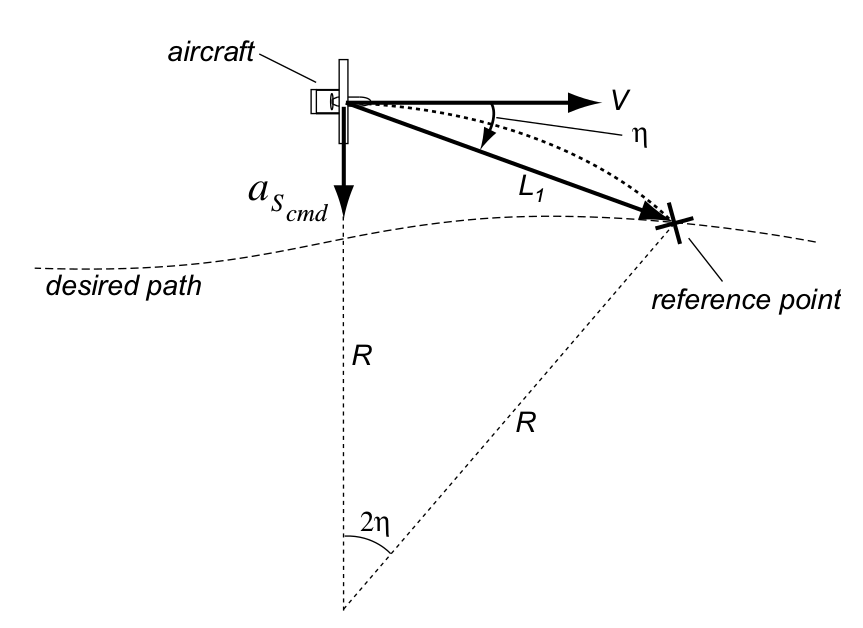
\includegraphics[width = 0.7\textwidth,trim = 0 -0 0 -0,clip]{L1.png}	  
	\caption{\label{fig: L1} L1轨迹跟踪计算示意图}
\end{figure}

通常轨迹跟踪都会针对直线轨迹和定点盘旋轨迹分别讨论。在直线轨迹跟踪中,侧偏距误差$d$可以用飞机质心与期望航线的垂直距离表示;在定点盘旋轨迹跟踪中,侧偏距误差$d$用飞机质心与圆的距离表示(质心到圆心距离 - 圆半径)。所以在应用L1轨迹跟踪算法时,需要考虑$d>L_1$的情况,也就是飞机距离轨迹较远的情况。

对于直线轨迹跟踪,在图\ref{fig: L1-line}中,可以对$\eta_1$进行限制,如$-30^\circ \le \rm{sat}(\eta_1) \le 30^\circ$。而对于盘旋轨迹,可以在$d>L_1$时先进行直线轨迹跟踪,期望直线可以取为过质心的圆切线(圆半径可适当增加一个差值),在$d<L_1$后再转入盘旋跟踪。另外在定点盘旋跟踪中需要利用速度向量与心心距向量判断旋转的方向(滚转的正负号)。

\begin{figure}[htbp]
	\figskip 
	\centering
	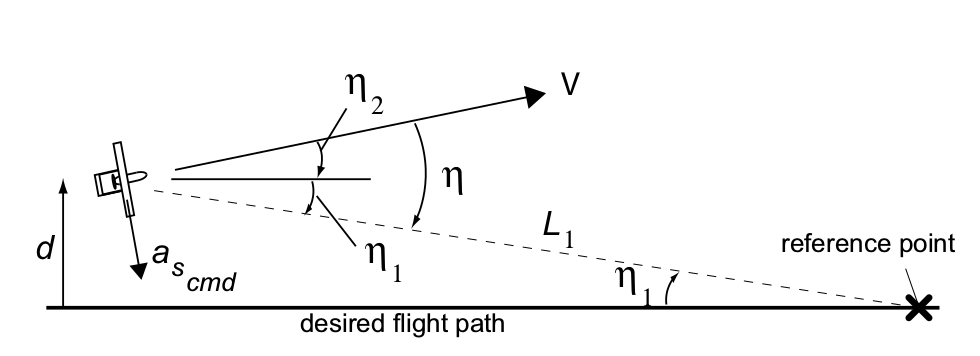
\includegraphics[width = 0.7\textwidth,trim = 0 -0 0 -0,clip]{L1-line.png}	  
	\caption{\label{fig: L1-line} 直线轨迹中L1轨迹跟踪计算示意图}
\end{figure}

在\href{attachment/L1t.m}{Matlab仿真}中验证定点盘旋算法时,通过几何关系可以直接计算$\eta$角度,再按原始公式计算加速度指令。而论文中则采用$\frac{V^2}{R} - \ddot{d}$进行近似,其中$\ddot{d}$在实现时似乎不方便计算。计算$\eta$角度时,涉及相交圆的求解,\href{http://blog.csdn.net/zx3517288/article/details/53326420}{参考这里的推导}。

最后,在L1算法中,给出了期望的加速度指令,如果假设飞机在进行高度不变的稳定盘旋时,侧向加速度指令等价于滚转角指令。而对于航向指令,论文中并没有提及,但是从PX4源码中可以看出,{\sout{直线轨迹时航向指令指向L1跟踪点,盘旋轨迹时航向指令始终指向圆心点}}两种轨迹下虽然给出了偏航指令,但在内环均保持协调转弯的偏航控制策略,而未跟踪该偏航角。
 
\subsection{进一步讨论}
以下讨论只针对固定翼,且假设1具有高度保持系统,2内环姿态控制的偏航通道按照协调转弯方式进行控制。多旋翼在做轨迹跟踪时,需要独立给出航向跟踪指令。

首先考虑偏盘旋轨迹跟踪问题,对于给定的飞行速度$V_a$和侧向加速度$a_s$(等价滚转角),在稳定盘旋时盘旋半径为$R = V_a^2 / a_s$。显然对于给定的盘旋半径,可以计算盘旋时的侧向加速度。如果以跟踪盘旋轨迹的圆心点作为参考点,那么无人机相对该参考点的运动可以分解为两部分:1.质心与圆心连线上的运动;2.相对圆心的圆周运动。若以侧向加速度为控制量,那么有

\begin{equation}
    a_{s_\rm{cmd}} = a_{\parallel} + a_{\perp} = \rm{f}(d,V_a) + \frac{V_a^2}{R}
\end{equation}
其中,$d$表示侧向轨迹偏差,$\rm{f}(d,V_a)$表示侧向偏差及飞行速度的函数,可以理解为对$d$的PD控制律。一种更形象的解释为:$a_{\perp}$能够让无人机产生一个指定半径的圆轨迹,$a_{\parallel}$能够让这个圆轨迹的圆心逐渐移动到指定的位置上。

\begin{figure}[htbp]
	\begin{minipage}[t]{0.5\textwidth}
	\centering
	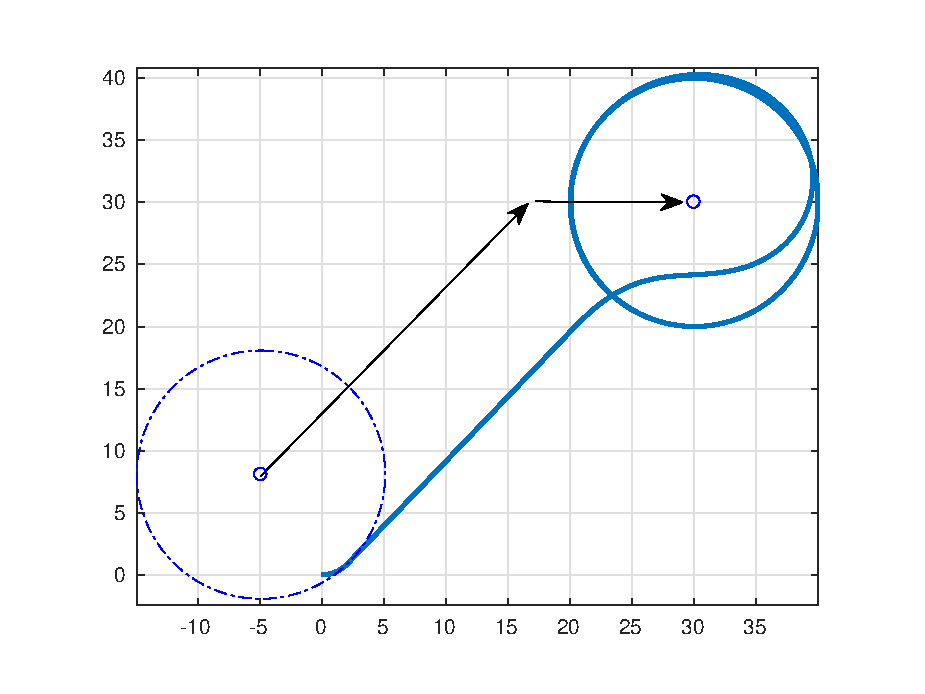
\includegraphics[width = 0.9\textwidth]{path1.eps}
	\caption{\label{fig: path1} 一种更形象的解释轨迹跟踪}
	\end{minipage}
	\begin{minipage}[t]{0.5\textwidth}
	\centering
	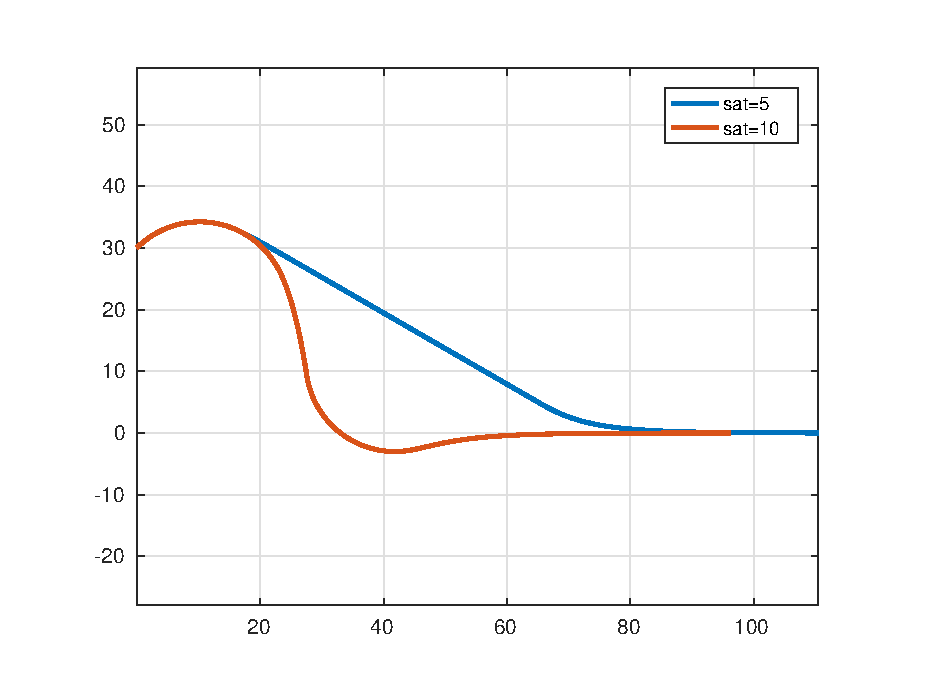
\includegraphics[width = 0.9\textwidth]{path2.eps}
	\caption{\label{fig: path2} 直线轨迹跟踪,对$d$取不同约束值的轨迹}
	\end{minipage}
\end{figure}


对于直线轨迹跟踪,可以认为是半径为$\infty$的圆轨迹,求解算法基本一致,只是需要在计算时限制$\rm{f}(d,V_a)$中的$d$值,以保证飞机能始终向前飞行,而不会对着航线飞行。

\subsection{其他的几种轨迹跟踪}
本节主要参考文献\href{attachment/Unmanned Aerial Vehicle Path Following.pdf}{\texttt{Unmanned Aerial Vehicle Path Following}}。


\section{MPC控制及动态路径跟踪}
模型预测控制(MPC)可以用于外环的路径跟踪控制上。若假设纵向控制中已经设计好了速度、高度控制器(比如TECS),且假设偏航控制能够按照协调转弯的方式保持飞机无侧滑,那么二维路径跟踪问题就可以转换成以侧向加速度/滚转角为输入量、以姿态闭环为被控系统的SISO控制问题。若内环控制器具有较好的控制性能,那么姿态闭环可以动态线性化为一个二阶串级线性系统,这时可以应用MPC进行控制。

MPC的核心问题就是在于对优化目标函数的设计及求解,若以师姐论文中的动态路径跟踪(避障)问题为例,优化目标函数可以设计为
\begin{equation*}
	J = \sum_i^N J^{(i)} = \sum_i^N \left(J_{path}^{(i)} + J_{angle}^{(i)} + J_{obs}^{(i)} + J_{final}^{(i)} \right)
\end{equation*}
其中,$N$为滚动优化的长度,$J^{(i)}$为滚动优化中每一步的罚函数,$J_{path}^{(i)}$为路径跟踪误差,$J_{angle}^{(i)}$飞行航向跟踪误差,$J_{obs}^{(i)}$为避障罚函数 + $J_{final}^{(i)}$为终点吸引罚函数。具体代码在\href{attachment/mympc.m}{\texttt{这里}}。运行的结果为:

\begin{figure}[htbp]
	\figskip 
	\centering
	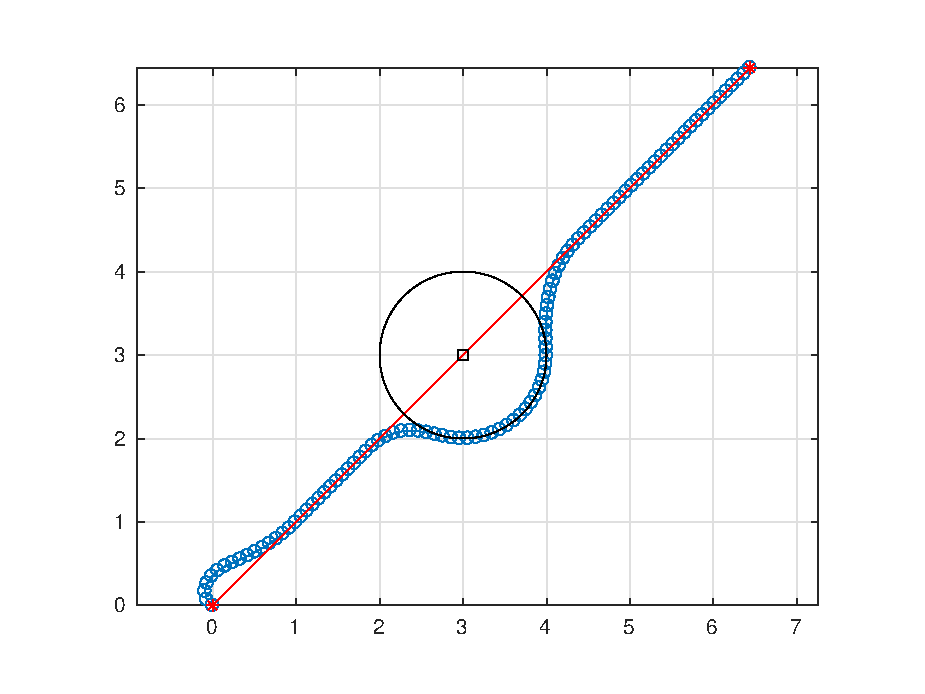
\includegraphics[width = 0.7\textwidth,trim = 0 -0 0 -0,clip]{mpc.eps}	  
	\caption{\label{fig: mpc} 一个简单的基于MPC的动态路径跟踪}
\end{figure}




\chapter{规划}
\section{最短路径算法}
\subsection{Floyd算法}
Floyd算法采用动态规划思想,$f[k][i][j]$表示$i$和$j$之间可以通过编号为$1 \dots k$的节点的最短路径。初值$f[0][i][j]$为原图的邻接矩阵。

则$f[k][i][j]$可以从$f[k-1][i][j]$转移来,表示$i$到$j$不经过$k$这个节点。也可以从$f[k-1][i][k]+f[k-1][k][j]$转移过来,表示经过$k$这个点。意思即
\begin{equation*}
	f[k][i][j] = \rm{min}(f[k-1][i][j], f[k-1][i][k]+f[k-1][k][j])
\end{equation*}

核心代码为
\begin{lstlisting}[language=c,numbers=left,firstnumber = 1,numberstyle=\tiny,breaklines = true,keywordstyle=\color{blue!70},commentstyle=\color{red!50!green!50!blue!50},frame=shadowbox, rulesepcolor=\color{red!20!green!20!blue!20}]
	for(k=1;k<=n;k++)
        for(i=1;i<=n;i++)
            for(j=1;j<=n;j++)
                if(e[i][j]>e[i][k]+e[k][j])
                     e[i][j]=e[i][k]+e[k][j];
\end{lstlisting}

Floyd算法能够求解有向图中任意两个点之间的最短路径,且只能在不存在负权环的情况下使用,时间复杂度$O(N^3)$,空间复杂度为$O(N^2)$。

\subsection{Dijkstra算法}
Dijikstra算法采用贪心思想,维护两个点集$A$,$B$。$A$点集代表已经求出源点到该点的最短路的点的集合,$B$代表未求出源点到该点的最短路径的点的集合。维护一个向量$d$,$d[i]$代表源点到点i的最短路径长度。不断进行以下操作:找出点集$B$中$d[i]$最小的点,将这个点加入点集A中,然后用这个点到其邻接点的距离来更新向量$d$,直到点集B为空。

\href{http://wiki.jikexueyuan.com/project/easy-learn-algorithm/dijkstra.html}{\texttt{具体步骤}}为:
\begin{enumerate}
\item 将所有的顶点分为两部分:已知最短路程的顶点集合 P 和未知最短路径的顶点集合 Q。最开始,已知最短路径的顶点集合 P 中只有源点一个顶点。我们这里用一个 book[ i ]数组来记录哪些点在集合 P 中。例如对于某个顶点 i,如果 book[ i ]为 1 则表示这个顶点在集合 P 中,如果 book[ i ]为 0 则表示这个顶点在集合 Q 中。
\item 设置源点 s 到自己的最短路径为 0 即 dis=0。若存在源点有能直接到达的顶点 i,则把 dis[ i ]设为 e[s][ i ]。同时把所有其它(源点不能直接到达的)顶点的最短路径为设为 ∞。
\item 在集合 Q 的所有顶点中选择一个离源点 s 最近的顶点 u(即 dis[u]最小)加入到集合 P。并考察所有以点 u 为起点的边,对每一条边进行松弛操作。例如存在一条从 u 到 v 的边,那么可以通过将边 u->v 添加到尾部来拓展一条从 s 到 v 的路径,这条路径的长度是 dis[u]+e[u][v]。如果这个值比目前已知的 dis[v]的值要小,我们可以用新值来替代当前 dis[v]中的值。
\item 重复第 3 步,如果集合 Q 为空,算法结束。最终 dis 数组中的值就是源点到所有顶点的最短路径。
\end{enumerate}

Dijkstra算法能够求解图中单源点到其他所有点的最短路径。时间复杂度为$O(|V|^2)$,$|V|$表示顶点个数。
如果采用优先队列,时间复杂度为$O(|E|+|V|\log|V|)$,$|E|$表示边数。

\begin{algorithm}[h] \caption{Dijkstra algorithm} 
\begin{algorithmic}[1] 
\FOR{each vertex $v \in V[G]$} 
\STATE d[v] := infinity
\STATE previous[v] := undefined
\ENDFOR

\STATE d[s] := 0      
\STATE S := empty set
\STATE Q := set of all vertices

\WHILE{Q is not empty}
\STATE u := Extract_Min(Q)
\STATE S.append(u)
\FOR{each edge outgoing from u as (u,v)}
\IF{d[v] > d[u] + w(u,v)}
\STATE d[v] := d[u] + w(u,v)
\STATE previous[v] := u
\ENDIF
\ENDFOR
\ENDWHILE

\end{algorithmic} \end{algorithm}


\subsection{Bellman-Ford算法}
\href{http://www.cnblogs.com/gaochundong/p/bellman_ford_algorithm.html}{\texttt{具体步骤}}为:
\begin{enumerate}
	\item 创建源顶点 v 到图中所有顶点的距离的集合 distSet,为图中的所有顶点指定一个距离值,初始均为 Infinite,源顶点距离为 0;
	\item 计算最短路径,执行V-1次遍历: 对于图中的每条边, 如果起点 u 的距离 d 加上边的权值 w 小于终点 v 的距离 d,则更新终点 v 的距离值 d;
	\item 检测图中是否有负权边形成了环: 遍历图中的所有边,计算 u 至 v 的距离,如果对于 v 存在更小的距离,则说明存在环;
\end{enumerate}

Bellman-Ford算法也能解决单源最短路问题,且对边的情况没有要求,不仅可以处理负权边,还能处理负环。时间复杂度为$O(|V|\cdot |E|)$

\subsection{A*算法}
个人理解A*算法只是针对搜索方向的一种启发式处理方法,在寻找最短路径的搜索过程中,通常都是以Dijkstra算法为基础进行的。具体的伪代码为:
\begin{lstlisting}[language=c,numbers=left,firstnumber = 1,numberstyle=\tiny,breaklines = true,keywordstyle=\color{blue!70},commentstyle=\color{red!50!green!50!blue!50},frame=shadowbox, rulesepcolor=\color{red!20!green!20!blue!20}]
function A*(start, goal)
    // The set of nodes already evaluated
    closedSet := {}

    // The set of currently discovered nodes that are not evaluated yet.
    // Initially, only the start node is known.
    openSet := {start}

    // For each node, which node it can most efficiently be reached from.
    // If a node can be reached from many nodes, cameFrom will eventually contain the
    // most efficient previous step.
    cameFrom := an empty map

    // For each node, the cost of getting from the start node to that node.
    gScore := map with default value of Infinity

    // The cost of going from start to start is zero.
    gScore[start] := 0

    // For each node, the total cost of getting from the start node to the goal
    // by passing by that node. That value is partly known, partly heuristic.
    fScore := map with default value of Infinity

    // For the first node, that value is completely heuristic.
    fScore[start] := heuristic_cost_estimate(start, goal)

    while openSet is not empty
        current := the node in openSet having the lowest fScore[] value
        if current = goal
            return reconstruct_path(cameFrom, current)

        openSet.Remove(current)
        closedSet.Add(current)

        for each neighbor of current
            if neighbor in closedSet
                continue		// Ignore the neighbor which is already evaluated.

            if neighbor not in openSet	// Discover a new node
                openSet.Add(neighbor)
            
            // The distance from start to a neighbor
            //the "dist_between" function may vary as per the solution requirements.
            tentative_gScore := gScore[current] + dist_between(current, neighbor)
            if tentative_gScore >= gScore[neighbor]
                continue		// This is not a better path.

            // This path is the best until now. Record it!
            cameFrom[neighbor] := current
            gScore[neighbor] := tentative_gScore
            fScore[neighbor] := gScore[neighbor] + heuristic_cost_estimate(neighbor, goal) 

    return failure

function reconstruct_path(cameFrom, current)
    total_path := [current]
    while current in cameFrom.Keys:
        current := cameFrom[current]
        total_path.append(current)
    return total_path
\end{lstlisting}
上述伪代码可以用于移动机器人路径搜索。其中closedSet表示已经搜索过的位置,openSet表示待搜索的位置。从openSet中按照fScore的值找到最近的待搜索点,从openSet中移入closedSet中。更新该点相邻可达点的fScore值和cameFrom表,同时将相邻点(不在closedSet)加入openSet中。不断重复直到搜索到达目标点,然后根据cameFrom表逆推得到最短路径。

与Dijkstra算法相比,A*算法最核心的地方就是对距离函数的取值:
\begin{equation*}
	f(n) = g(n) + h(n)
\end{equation*}
其中,$g(n)$就是Dijkstra算法中计算出的从源点到当前点的距离,$h(n)$则表示当前点到目标点的距离估计。常见的估计函数有:欧几里得距离、曼哈顿距离、切比雪夫距离;这个公式遵循以下特性:
\begin{enumerate}
\item 如果$g(n)$为0,则转化为使用贪心策略的深度优先搜索,速度最快,但可能得不出最优解;
\item 如果$h(n)$为0,则转化为单源最短路径问题,即Dijkstra算法;
\item {\color{red} 如果$h(n)$不大于顶点$n$到目标点的真实距离,则一定可以求出最优解}。而且$h(n)$越小,需要计算的节点越多,算法效率越低。
\end{enumerate}

利用该估计值启发搜索方向。这是我用Matlab编写的\href{/attachment/myastar.m}{\texttt{A*代码}}。为了便于Matlab搜索和定位,代码中将二维坐标转换为了一维坐标处理。

\section{路径搜索算法}
\subsection{PRM算法}
概率路图(Probabilistic RoadMap, PRM)算法。基本步骤分为两步:先对地图进行预处理建图,生成可行路径无向图,然后查询源点、终点在图上对应的最短距离。

\noindent {\hei $\blacksquare$ PRM算法预处理步骤}

\begin{enumerate}
\item 地图随机采样,生成中间路径点。
\item 按照不同的方法,在路径点之间生成路径
\item 对路径进行碰撞检测。
\end{enumerate}

在PRM算法中,常规方式是逐点采样,然后按照半径距离$r$连接到已生成的图中;一种简化方法(sPRM)是一次生成N个采样点,然后再逐点生成路径。此外,对最近若干点的挑选方式也有不同处理。常规是按照给定的半径球内寻点。k-Nearest (s)PRM 始终搜寻最近的k个点生成路径。Bounded-degree (s)PRM 则是对常规方式的球内点添加了k个最近上限。


\subsection{RRT算法}
快速扩展随机树(Rapidly-exploring Random Trees, RRT)算法。本节主要参考\href{http://rkala.in/codes/RRT.zip}{\texttt{Rahul Kala}}的代码以及\href{http://www.cnblogs.com/21207-iHome/p/7210543.html}{\texttt{这篇博客}}。

\noindent {\hei $\blacksquare$ RRT算法步骤}

\begin{enumerate}
\item 初始化随机树,确定初始点、目标点,地图尺寸、地图障碍物位置等
\item 随机采样。按照一定的概率在地图中挑选随机点或是用目标点作为当前采样点$q_\rm{rand}$
\item 选取最近节点。在当前随机树中找出与采样点最近的节点,作为扩展节点$q_\rm{nearest}$
\item 随机树扩展。沿$q_\rm{nearest}$和$q_\rm{rand}$方向,按照一定步长生成新节点$q_\rm{new}$
\item 碰撞检测。若$\overrightarrow{q_\rm{nearest} q_\rm{new}}$上的点都与障碍物无碰撞,则将$q_\rm{new}$加入随机树中。
\item 若$q_\rm{new}$距离目标点足够近则停止搜索,否则跳转步骤2。
\end{enumerate}

在实际使用是,还需要考虑:如何进行随机采样?如何定义“最近”以及如何快速搜索到最近节点(Kd-Tree)?如何进行扩展等。博客中举了一个车型机器人的例子,显然车的前后移动要比旋转、航向移动要方便,对应与更“近”。

\noindent {\hei $\blacksquare$ Bidirectional RRT/RRT Connect}

单源点开始搜索的RRT算法在搜索效率上仍显的较慢,因此有人提出如下的双向RRT搜索算法。
\begin{figure}[htbp]
	\figskip 
	\centering
	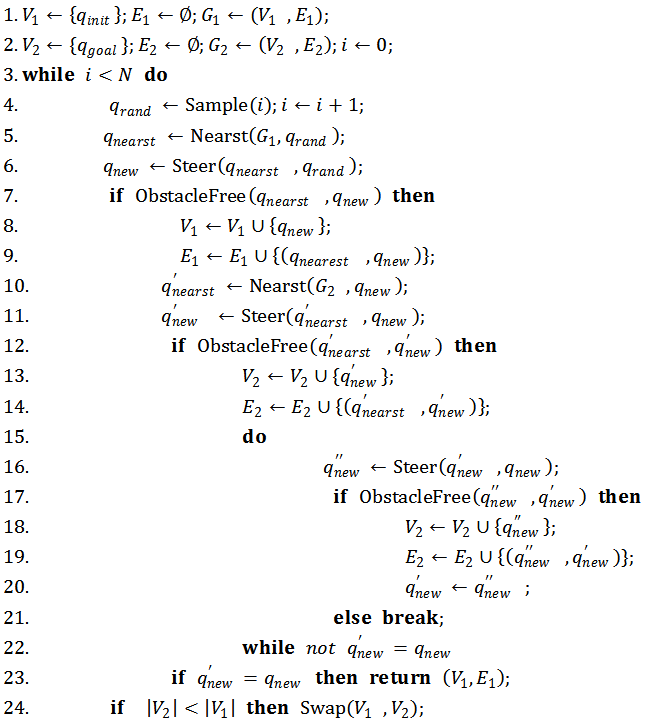
\includegraphics[width = 0.85\textwidth,trim = 0 -0 0 -0,clip]{rrt-connect.png}	  
	\caption{\label{fig: rrt-connect} RRT-Connect算法步骤}
\end{figure}
基本思想可以理解为:先对源点做一次RRT搜索,然后用扩展点对终点做一次RRT搜索,然后用源点RRT的扩展点与终点RRT的扩展点再做连续RRT拓展,直到遇到障碍物。然后重复上述步骤。为了平衡两棵随机树的节点,每一步搜索中的第一次的RRT可以对节点数多的进行。

\subsection{RRT*算法}
最优RRT(RRT*)算法,主要参考\href{/attachment/Sampling-based Algorithms for Optimal Motion Planning10.1.1.419.5503.pdf}{\texttt{这篇论文}}。简单来说,RRT*算法的“最优”性体现在对随机树的动态优化上,基本思想为:

\begin{enumerate}
    \item 随机树扩展。对于待扩展的新节点$q_\rm{new}$,不是简单的生成从$q_\rm{nearest}$到$q_\rm{new}$的路径,而是在$q_\rm{new}$的一个邻域内搜索所有节点$q_\rm{near}$,使得源点经过$q_\rm{near}$到$q_\rm{new}$的路径最短,这时再添加$q_\rm{near}$到$q_\rm{new}$路径。
    \item 随机树修正。对$q_\rm{new}$邻域内所有节点$q_\rm{near}$再做一次搜索,若源点经过新节点$q_\rm{new}$到$q_\rm{near}$的距离更短,则变更$q_\rm{near}$的父节点为$q_\rm{new}$,且替换原路径。
\end{enumerate}

\begin{figure}[htbp]
	\figskip 
	\centering
	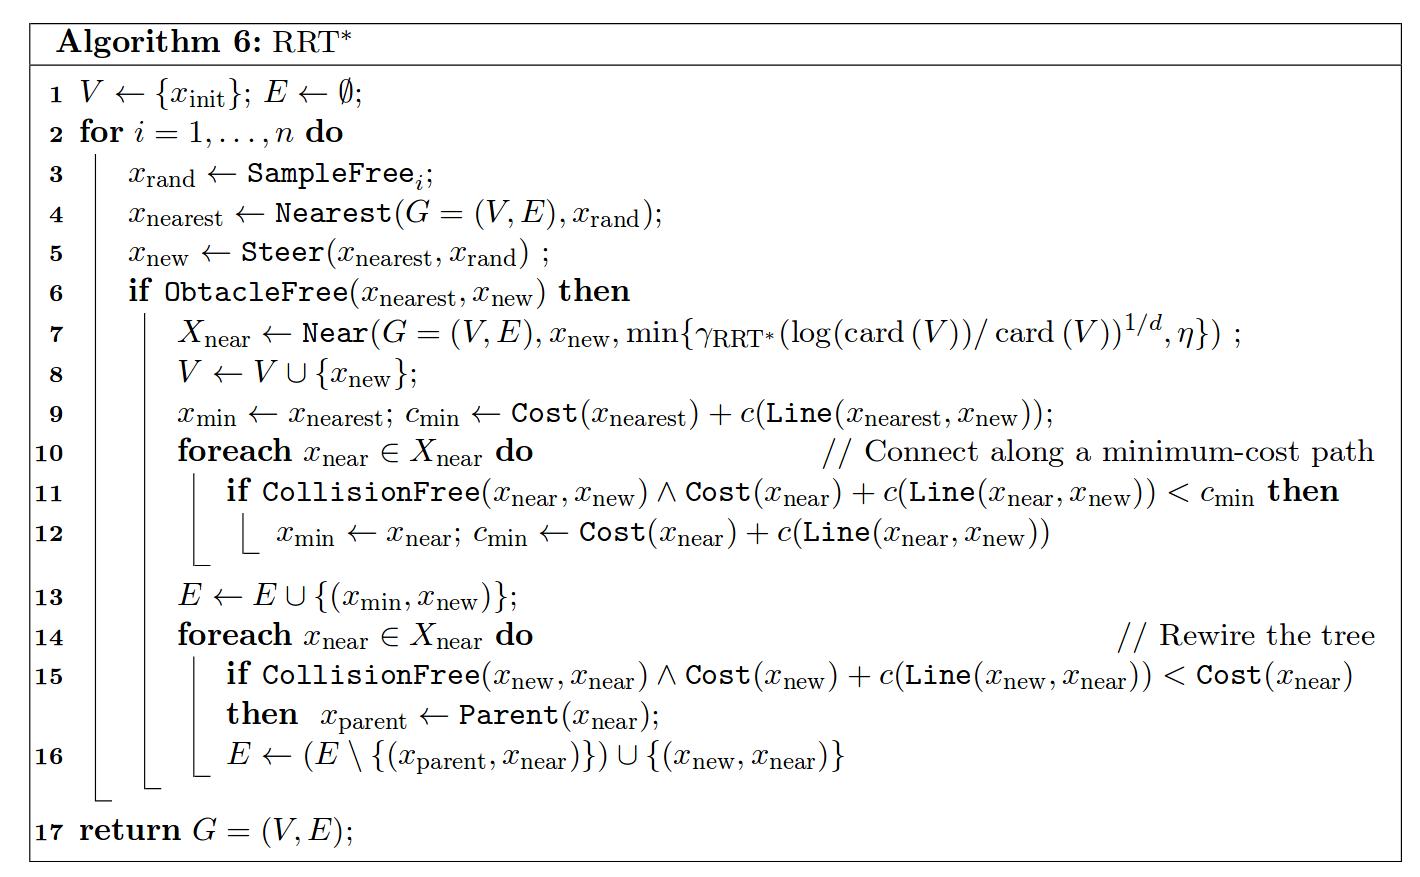
\includegraphics[width = 0.9\textwidth,trim = 0 -0 0 -0,clip]{RRT*.png}	  
	\caption{\label{fig: RRT*} RRT*算法伪代码}
\end{figure}

\noindent {\hei $\blacksquare$ 疑问}

RRT*算法在每一步搜索中都需要寻找$q_\rm{new}$的邻域节点,这个搜索的代价是不是太大?如果按照常规RRT算法生成节点和路径,最后再做一次全局的最短路径搜索,性能对比如何?

\section{路径曲线生成算法}
\subsection{Dubins path}
对于平面路径生成,可以用$(x,y,\psi)'$表示状态,其中$x,y$为轨迹点的平面坐标位置,$\psi$表示轨迹点运动的轨迹偏角(对无人机,假设无侧滑角飞行)。Dubins曲线采用圆弧和直线连接源点和终点,对于包含直线的Dubins曲线,按照源点转弯方向和终点转弯方向,可以分为RSR,RSL,LSR,LSL共四种曲线形式。

\begin{figure}[htbp]
	\figskip 
	\centering
	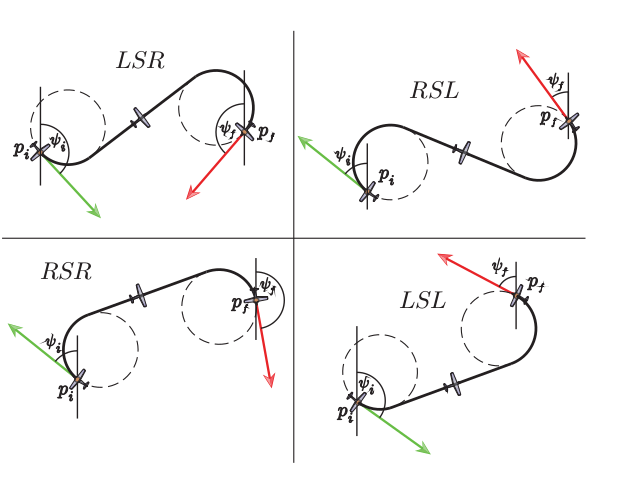
\includegraphics[width = 0.75\textwidth,trim = 0 -0 0 -0,clip]{Dubins.png}	  
	\caption{\label{fig: Dubins} 四种Dubins曲线形式}
\end{figure}

具体算法思想可以参考\href{/attachment/Dubins.pdf}{\texttt{这篇论文}},具体的MATLAB实现可以看
\href{/attachment/dubins.m}{\texttt{这里}},主要注意下坐标系(x轴指向北)与论文中不一样,实现过程比较简单,都是几何运算。

基本思路都是:
\begin{enumerate}
	\item 按照路径形式确定源点、终点的转弯圆心
	\item 按照路径形式确定两圆的切线方向、航迹偏角
	\item 计算圆上切点
	\item 计算转弯旋转角度的变化增量
\end{enumerate}

关于如何根据条件状态直接选择路程最短的形式,可以参考王师姐论文。

\subsection{Bezier曲线 和 B-spline曲线}
\noindent {\hei $\blacksquare$ 贝塞尔曲线}

参考\href{https://www.cnblogs.com/hnfxs/p/3148483.html}{\texttt{这篇博客}}。给定源点$P_0$和终点$P_1$,那么一阶Bezier曲线就是这两个点的连线,连线上的点可以描述为:
\begin{equation*}
    P = (1-t)P_0 + tP_1
\end{equation*}
其中,$t: 0 \Rightarrow 1$。这个形式相当于一个一阶插值。类似的,二阶Bezier曲线中,一共需要3个控制点$P_0$,$P_1$,$P_2$,先计算$P_0$和$P_1$的曲线点$P_0^1$,再计算$P_1$和$P_2$的曲线点$P_1^1$,最后计算$P_0^1$和$P_1^1$的曲线点就是二阶曲线上的点。

\begin{align*}
    P &= (1-t)\left[(1-t)P_0 + tP_1\right] + t\left[ (1-t)P_1 + tP_2\right] \\
      &= (1-t)^2 P_0 + 2t(1-t)P_1 + t^2 tP_2
\end{align*}

贝塞尔曲线存在的问题:
\begin{enumerate}
	\item 确定了多边形的顶点数(m个),也就决定了所定义的Bezier曲线的阶次(m-1次),不够灵活。
    \item 当顶点数(m)较大时,曲线的阶次将比较高。此时,多边形对曲线形状的控制将明显减弱。    
    \item Bezier的调和函数的值,在开区间(0,1)内均不为0。因此,所定义的曲线在(0<t<1)的区间内的任何一点均要受到全部顶点的影响,即改变其中任一个顶点的位置,都将对整条曲线产生影响,因此对曲线进行局部修改是不可能的。
\end{enumerate}

\noindent {\hei $\blacksquare$ B样条曲线}

可以参考\href{https://blog.csdn.net/Mr_Grit/article/details/45603627}{\texttt{这篇博客}}。讲的比较清楚,而且代码也可以运行通过。

一般使用其中的准均匀B样条曲线,需要特别注意其中求取节点的地方,包括数量及其分布。节点可以理解为在原控制点上的扩充,用于计算基函数。控制点就是给定的控制多边形的定点。




\subsection{其他形式曲线}
\noindent {\hei $\blacksquare$ Reeds-Shepp曲线}

与Dubins曲线相比,RS曲线中机器人既能够前向运动,也能够后向运动(类似具有倒车的性质)。共计9类46种曲线直线组合结果。

\noindent {\hei $\blacksquare$ Balkcom-Mason曲线}

与RS曲线相比,Balkcom-Mason曲线中机器人可以绕中心旋转(类似双轮机器人差动转向的性质)。

\noindent {\hei $\blacksquare$ Pythagorean Hodograph曲线}

PH曲线是一种具有有理特性的参数化多项式曲线。具体计算可以根据师姐论文中的方法,在复平面内进行计算。

\subsection{多项式轨迹}
通过路径搜索算法可以找到一系列的离散路径点,通过多项式曲线将这些点连接起来形成多项式轨迹。本节的主要算法参考\href{https://pdfs.semanticscholar.org/2376/078d13761387cabb933798b93a706c2ea7ef.pdf}{\texttt{论文A}}
和\href{http://www-personal.acfr.usyd.edu.au/spns/cdm/papers/Mellinger.pdf}{\texttt{论文B}}。其中对于多项式轨迹的基本内容可以阅读教材 Trajectory Planning for Automatic Machines and Robots Springer 第二章中的相关部分。

对于本节的多项式轨迹生成问题,可以转化为求解一个二次规划(QP, Quadratic Program)问题。
假设多项式的系数可以表示为$\bm{p} = [p_0, p_1, \cdots, p_n]^T$,多项式函数为$P(t)$ 那么采用论文A中的目标函数:

\begin{equation}
    J(T) = \int_0^T c_0 P(t)^2 + c_1 P'(t)^2 + c_2 P''(t)^2 + \cdots + c_N P^{(N)}(t)^2 \dd t = \bm{p}^T Q(T) \bm{p}
\end{equation}
其中,$Q(T)$ 为Hessian矩阵,可以通过简单的微积分运算求解。$T$表示每一段多项式轨迹的总时间。
对于M+1个离散路径点,共需要生成M段多项式轨迹,这样总的目标函数可以表示为:

\begin{equation}
J_{total} = \begin{bmatrix} \bm{p}_1 \\ \vdots \\ \bm{p}_M \end{bmatrix}^T 
 \begin{bmatrix} Q_1(T_1) & & \\ & \ddots & \\ & & Q_M(T_M) \end{bmatrix}
 \begin{bmatrix} \bm{p}_1 \\ \vdots \\ \bm{p}_M \end{bmatrix}^T 
\end{equation}

对于二次规划问题可以通过现成的工具箱进行求解,所以剩下的问题就是如何将轨迹生成中的边界约束转化为二次规划的约束形式。
{\color{red}此外需要注意的是上述目标函数中需要指定每一段的轨迹时间,这些时间量可以作为上一层优化问题的优化变量。}

从无人机飞行动力学考虑,一种合理的假设是飞行过程中无人机位置、速度、加速度是连续变化的,每一段的边界条件也是位置、速度、加速度这三个变量。
那么对于任意一段多项式轨迹,初始边界条件3个,终端边界条件3个,因此需要最少5次多项式(6个系数)才能满足所有边界条件。对每一段多项式的边界条件可以描述为:
\begin{equation}
    \bm{A}_i \bm{p}_i = \bm{d}_i
\end{equation}
对于5次多项式,考虑P、V、A三项边界时,上述三项展开为:
\begin{equation}
    \bm{A}_i = \begin{bmatrix}
        1   & t_0   & t_0^2     & t_0^3     & t_0^4     & t_0^5 \\
        0   & 1     & 2 t_0     & 3 t_0^2   & 4 t_0^3   & 5 t_0^4 \\
        0   & 0     & 2         & 6 t_0     & 12 t_0^2  & 20 t_0^3 \\
        1   & t_T   & t_T^2     & t_T^3     & t_T^4     & t_T^5 \\
        0   & 1     & 2 t_T     & 3 t_T^2   & 4 t_T^3   & 5 t_T^4 \\
        0   & 0     & 2         & 6 t_T     & 12 t_T^2  & 20 t_T^3 
    \end{bmatrix}
\end{equation}

\begin{equation}
    \bm{d}_i = [P_0, \, V_0, \, A_0, \, P_T, \, V_T, \, A_T]^T
\end{equation}

在实际规划过程中,常常并不知道无人机到达中间离散路径点位置时的速度、加速度,因此需要使用连续边界条件,即
\begin{equation}
    A_{T,i} \bm{p}_i = A_{0,i+1} \bm{p}_{i+1}
\end{equation}





\chapter{LeetCode}
\section{数论}
\subsection{Power of Three}

\noindent {\hei $\blacksquare$ \href{https://leetcode.com/problems/power-of-three/description/}{\texttt{题目描述}}}:

给一个整数,判断是否为3的整数幂。要求不使用循环/递归。

\noindent {\hei $\blacksquare$ 解答思路一}:

若整数$N$是3的整数幂,即$3^a = N$ 那么$a = \log_3 N$一定也是一个整数,使用换底公式为:
\begin{equation*}
    a = \frac{\log_{10} N}{\log_{10} 3} 
\end{equation*}
注,不能使用自然对数$e$或2为底进行计算,无法通过。
判断$a$是否为整数可以用\texttt{(a - (int)a == 0)}来判断。

\noindent {\hei $\blacksquare$ 解答思路二}:

可以用int范围内最大的一个3的整数幂来求余,若余数为0,表明$N$是3的整数幂。

\section{树}
\subsection{Recover Binary Search Tree}

\noindent {\hei $\blacksquare$ \href{https://leetcode.com/problems/recover-binary-search-tree/description/}{\texttt{题目描述}}}:

给一个二叉搜索树,其中有两个节点位置交换了,需要将其恢复。要求空间复杂度为O(N)。

\noindent {\hei $\blacksquare$ 解答思路}: \\
1. 先序遍历二叉搜索树时,遍历结果为一个递增序列。若出现某个元素大于后一个元素,则说明这两个元素的位置有误。\\
2. 要求只使用O(N)空间复杂度,所以不能用常规递归/迭代的方式进行遍历,需要使用Morris traversal的遍历方式。具体算法为:\\

A...如果左子树为空,打印当前节点,并将当前节点指向右子树。

B...如果左子树非空,迭代找到左子树中的先序遍历的最后一个节点。

.......a) 如果该节点的右子树指向当前节点,则将恢复右子树为NULL,当前节点指向右子树。

.......b) 如果该节点的右子树为空,则将右子树指向当前节点,打印当前节点,并将当前节点指向左子树。

C...迭代重复上述过程直到当前节点为空。

\noindent 3. 需要将上述算法中节点打印的顺序用一个指针记录。

\begin{lstlisting}[language=c++,numbers=left,firstnumber = 1,numberstyle=\tiny,breaklines = true,keywordstyle=\color{blue!70},commentstyle=\color{red!50!green!50!blue!50},frame=shadowbox, rulesepcolor=\color{red!20!green!20!blue!20}]
struct TreeNode {
    int val;
    TreeNode *left;
    TreeNode *right;
    TreeNode(int x) : val(x), left(NULL), right(NULL) {}
};

int MorrisTravelPreorder(TreeNode* root){
    TreeNode *cur = root;
    TreeNode *pre = NULL;
    while(cur){
        if (!cur->left) {
            cout << cur->val << endl;
            cur = cur->right;
        } else {
            pre = cur->left;
            while(pre->right && pre->right != cur){
                pre = pre->right;
            }
            if (!pre->right) {
                pre->right = cur;
                cur = cur->left;
            } else {
                pre->right = NULL;
                cout << cur->val << endl;
                cur = cur->right;
            }
        }
    }
}
\end{lstlisting}
\backmatter


% 参考文献
\defaultfont
% \bibliographystyle{GBT7714-2005_2}
% \bibliography{body/reference}
% \addcontentsline{toc}{chapter}{参考文献}
\cleardoublepage




\defaultfont


% 版权页
% \phantomsection  % 让 hyperref 宏包生成的链接指向正确的位置

\end{document}